\section{Mapping the MTConnect Information Model to OPC UA} 
  \label{mtconnect-mapping}

This section describes a UML representation of MTConnect semantic data models for mapping MTConnect into OPC UA. More detailed information is provided in Section \ref{mtconnect_information_model} for each data type.

OPC UA defines abstractions representing data, relationships, and events from devices. The abstractions do not provide the semantic meaning; they provide a structure to convey the meta-data and the values as they change. The OPC UA model has the base building blocks to represent an ontological model where the specific ontology is povided by companion specification for a specific domain.

MTConnect has similar facilities but uses different structural model where the meta-data and the streaming values are in separate documents to normalize the data flow in a similar way that many publish-subscribe protocols separate the structure from the data. MTConnect also supports a store-and-forward capability like many message brokers in a Message Oriented Middleware \textit{(MOM)} architecture to enable resilience and recovery of data in the event of connectivity problems.

When translating from MTConnect to OPC UA, the MTConnect abstractions of \mtconnectterm{DataItem}s are converted using the OPC UA  \opcuaterm{DataVariable} abstractions as given in \cite{UAPart8}.  The relationships are mapped to multiple \opcuaterm{DataVariable} types where the category and the type determine the correct mapping. Conditions are mapped a sub-type of the OPC UA \opcuaterm{ConditionType} in a similar way. The behavior of the OPC UA \opcuaterm{Condition}s can be found in \cite{UAPart9}.

\subsection{MTConnect UML Representation of OPC}

This section provides instructions to translate from the OPC UA diagram representation given in section \ref{intro-to-opc-ua} to the UML described throughout section \ref{mtconnect-mapping}. Figure \ref{fig:mtcomponent-ua} is a partial illustration of the MTConnect \mtconnectterm{Component} abstraction in OPC UA.

\begin{figure}[ht]
\centering\scalebox{0.8}{
\begin{tikzpicture}[auto]

\ObjectType{MTComponentType}{}{}{}{};
\Object{<Component>}{left of}{MTComponentType}{4.5}{};
\HasTypeDefinition{}{<Component>}{--}{MTComponentType}{};

\ObjectType{NTDeviceType}{right of}{MTComponentType}{4.5}{};
\HasSubType{}{NTDeviceType}{--}{MTComponentType}{};

\Variable{XmlId}{below right of}{MTComponentType}{3.5}{};
\Variable{Name}{below of}{XmlId}{2}{};
\Variable{NativeName}{below of}{Name}{2}{};
\Variable{Uuid}{below of}{NativeName}{2}{};
\Variable{SampleRate}{below of}{Uuid}{2}{};
\Variable{SampleInterval}{below of}{SampleRate}{2}{};

\HasProperty{}{MTComponentType}{|-}{XmlId}{};
\HasProperty{}{MTComponentType}{|-}{Name}{};
\HasProperty{}{MTComponentType}{|-}{NativeName}{};
\HasProperty{}{MTComponentType}{|-}{Uuid}{};
\HasProperty{}{MTComponentType}{|-}{SampleRate}{};
\HasProperty{}{MTComponentType}{|-}{SampleInterval}{}l

\Object{Description}{below left of}{MTComponentType}{3.5}{};
\HasComponent{}{MTComponentType}{|-}{Description}{};

\Object{Configuration}{below of}{Description}{2}{}
\HasComponent{}{MTComponentType}{|-}{Configuration}{};

\end{tikzpicture}
}
\caption{MTConnect MTComponentType in OPC UA}
 \label{fig:mtcomponent-ua}
\end{figure}



Figure \ref{fig:mtcomponent-uml} represents the same model in UML. The companion specification uses the following conventions:

\begin{itemize}
\item OPC UA Types are represented as \mtterm{UML Classes}
\item OPC UA Objects are represented as ``\uaterm{BrowseName}: \uaterm{Type}'' underlined as in the following example: \textbf{\underline{SimpleCnc: MTDeviceType}} where \textbf{\underline{SimpleCnc}} is the name of the device and  \textbf{\underline{MTDeviceType}} is related with a \uaterm{HasTypeDefinition} relationship.
\item Stereotypes are used to denote properties of types, relationships, and members of types. A stereotype is denoted by angle brackets (\texttt{<<..>>}) and provides additional information about the entity. For example, each reference from one \uaterm{ObjectType} to another has a stereotype denoting the reference type.
\item OPC UA Properties are denoted as UML Attributes. UA \uaterm{Attributes} are also represented as UML Attributes with the stereotype of \mtconnectterm{<<attribute>>} to differentiate from UA \uaterm{Properties}.
\item OPC UA \uaterm{Component} \uaterm{References} are represented as UML Unidirectional associations. The reference type is given as the association's \textit{Stereotype}, for example \textit{<<HasComponent>>}. 
\item \uaterm{HasSubtype} relationships are given as an UML Generalization association.
\item Combinining of templates and classes can be done using a UML \mtterm{Realization} with the stereotype \mtterm{<<Mixes In>>} to use common properties and relationships in a collection of otherwise unrelated types.
\end{itemize}

The \mtterm{UML Associations} are used to represent OPC UA R`eferences. \uaterm{UA Properties} represented using the UA \opcuaterm{HasProperty} relationships are given as UML Attributes (not be confused with the \uaterm{OPC UA Attribute}). UML allows for additional information as follows:  the multiplicity of a property, the data type of the property, are specified.

\begin{figure}[ht]
\centering\scalebox{0.8}{
\begin{tikzpicture}[auto]

\umlabstract[x=0, y=0]{MTComponentType}{
+ XmlId: String \\
+ Name: String[0..1] \\
+ NativeName: String[0..1] \\
+ Uuid: String[0..1] \\
<<Deprecated>> + SampleRate: Float[0..1] \\
+ SampleInterval: Float[0..1] \\
}{}

\umlclass[right=1.5cm of MTComponentType]{MTDeviceType}{
+ Version: String[0..1] \\
<<Deprecated>> + Iso841Class: String[0..1] \\
}{}

\umlinherit[geometry=--]{MTDeviceType}{MTComponentType}

\umlclass[below left=1cm and 2cm of MTComponentType.south]{DescriptionType}{
+ Station: String[0..1] \\
+ SerialNumber: String[0..1] \\
+ Manufacturer: String[0..1] \\
+ Data: String[0..1] \\
}{}

\umluniassoc[geometry=-|,stereo=HasComponent,%
              arg1=Description,pos1=0.5,pos2=1.8,%
              pos stereo=1.4,anchor2=140,%
              mult1=0..1,%
              mult2=1]{MTComponentType}{DescriptionType}

\umlsimpleclass[below=1cm of MTDeviceType.south]{<Component>Type}
\umlinherit[geometry=-|-,arm2=4.5cm]{<Component>Type}{MTComponentType}

\umlabstract[below right=2.5cm and -0.1cm of MTComponentType.south]{MTConfigurationType}{}{}

\umluniassoc[stereo=HasComponent,pos1=.2,%
              arg1=Configuration,anchor1=-60,anchor2=130,%
              mult1=0..1,%
              mult2=1]{MTComponentType}{MTConfigurationType}
              
\umlclass[below=1cm of MTConfigurationType.south]{SensorConfigurationType}{
+ FirwareVersion: String[0..1] \\
+ CalibrationDate: UtcTime[0..1] \\
+ NextCalibrationDate: UtcTime[0..1] \\
+ CalibrationInitials: String[0..1] \\
}{}

\umlinherit[geometry=-|]{SensorConfigurationType}{MTConfigurationType}

\end{tikzpicture}
}
\caption{MTConnect MTComponentType in UML}
 \label{fig:mtcomponent-uml}
\end{figure}

\FloatBarrier

When traversing an association between two object types, the name of the source of the association is the browse name associated with the object, and the destination is the type of object that is instantiated. If the name is not given, it represents a dynamic relationship where the browse name is determined during the creation of the object model. An example is the association of the MTConnect \mtconnectterm{DataItem}s.

A reference that has a stereotype of \textit{<<Organizes>>}, shown by the \texttt{Components} recursive relationship in the \mtconnectterm{MTComponentType}, implies an intermediate object of type \opcuaterm{FolderType} with the \uaterm{BrowseName} of the relationship point on the source side. The far side is not constrained within the \opcuaterm{FolderType} but given in the documentation as the expected contents of the folder.

OPC UA represents both class and instance diagrams using the same set of primitives. UML provides separate class and object models using two separate sets of primitives, one for classification and the other for instances of those classes. This section separates the object instantiation from the classification and uses UML object diagrams to represent example instances of classes.

\FloatBarrier

\subsubsection{MTConnect UML Object Model}

The object models will use a UML representation that represents the members as UML Slots. There is no distinction between an attribute and a property; consult the type model for the proper associations.

\begin{figure}[ht]
\centering\scalebox{0.8}{
\begin{tikzpicture}[node distance=1.5cm, font=\small]
\tikzset{
   object/.style={
           rectangle,
           rounded corners,
           draw=black, very thick,
           minimum height=2em,
           inner sep=2pt,
           text centered           
           },
}

\node[object] (device) { %
\begin{tabular}{l l}
  \multicolumn{2}{c}{\underline{\textbf{SimpleCnc: \typeref{MTDeviceType}}}} \\[4pt]
  \hline
  NodeId & ""872a3490-\ldots" \\
  XmlId & "x872a3490" \\
  Name & "SimpleCnc" \\
  Uuid & "872a3490-\ldots" \\ 
 \end{tabular}
};

\node[object,right=3cm of device] (server) { %
\begin{tabular}{l l}
  \multicolumn{2}{c}{\underline{\textbf{Server: ServerType (OPC)}}} \\[4pt]
 \end{tabular}
};

\node[object,below=2cm of device] (description) { %
\begin{tabular}{l l}
  \multicolumn{2}{c}{\underline{\textbf{Description: \typeref{MTDescriptionType}}}} \\[4pt]
  \hline
  NodeId & "e0d67070" \\
  Manufacturer & "MTConnectInstitute" \\
  Model & "Simple" \\
  SerialNumber & "12" \\ 
  Data & "This is a simple CNC example" \\
 \end{tabular}
};

\draw[->,thick] (device) -- (description)
  node[pos=0.5,right]{<<HasComponent>>};

\draw[->,thick] (server) -- (device) 
  node[pos=0.5,below]{<<HasNotifier>>};

\end{tikzpicture}
}
\caption{MTConnect Example Object}
 \label{fig:example-object}
\end{figure}

Figure \ref{fig:example-object} represents an MTConnect \mtconnectterm{Device} with the values filled in. The UA \opcuaterm{Browse\-Name} is given as the object name above, and the UA Type is given after the \texttt{:} in the header. Each of the UA \opcuaterm{Attributes} and \opcuaterm{Properties} are provided below. Relationships are shown as edges that have the Reference Type, such as \opcuaterm{Has\-Component}. The properties contained within will be created using the \opcuaterm{Has\-Property} reference but composed as internal members for brevity.

For example, the with type \mtuatype{MTDeviceType} has \opcuaterm{BrowseName} of \texttt{SimpleCnc} (the name of the device). There are patterns for creating all the \uaterm{BrowseName} for each MTConnect UA Type. The rules are presented and in the example to provide the normative patterns for each type in the information model.

\begin{quote}
    \color{red} Dcoument conventions for browse names on edges. Object identity vs. Browse Name. May not be an issue when UML diagrams are converted to Tikz.
\end{quote}

\FloatBarrier

\subsection{MTConnect Information Model}

The MTConnect information model has the following abstractions:

\begin{enumerate}
\item \mtconnectterm{Components}
\item \mtconnectterm{DataItems}
\item \mtconnectterm{Configuration}
\item \mtconnectterm{Compositions}
\item \mtconnectterm{Assets}
\end{enumerate}

The first concern of the MTConnect OPC UA companion specification is the \mtterm{Device} model covered in MTConnect \cite{MTCPart2} and \cite{MTCPart3}. The top-level \mtconnectterm{Component} of any MTConnect information model is the \mtconnectterm{Device}. A \mtconnectterm{Component} represents a logical part or a collection of parts of a piece of equipment. The \mtconnectterm{DataItem}s represent information that is communicated from \mtconnectterm{Component}s, and the representation and communication of the information are covered in \cite{MTCPart3}. The \mtconnectterm{Compositions} are the lowest level of contextualization for MTConnect \mtconnectterm{Components} that do not have any structure but can be associated with \mtconnectterm{Data\-Item}s to provide additional context. 

The \mtconnectterm{Configuration} is a collection of information about the component that provides more detail about its capabilities. The standard has only specified the \mtconnectterm{SensorConfiguration} at this point.

\mtconnectterm{Asset}s are complex information models that provide a point in time consistent set of information about the use of a physical or logical entity in the manufacturing process. These models, for example, may represent a cutting tool, a program, or a process. The \mtconnectterm{Asset}s will be covered in a subsequent companion specification. The only assets currently in the MTConnect standard are \asset{CuttingTool} and \asset{CuttingToolArchetype}. Refer to MTConnect Part 4.0 \cite{MTCPart40} and MTConnect Part 4.1 \cite{MTCPart41}.

The specification uses examples to illustrate the process of conversion from XML to OPC UA; the following sections cover the main points and concerns when converting an MTConnect Device model to a Nodeset. Following the metamodel discussion will be a section on the handling of streaming data and mapping to the correct data items. 

\subsection{Mapping The Model}
\lstset{language=XML,numbers=left,xleftmargin=2em}

The MTConnect information model is represented in the UA address space as set of object and variable types. Most have pre-existing type definitions whereas others will be created dynamically following riles in the following section. The rules provide a way for a developer of a server to extend the nodeset to include the types present in a given MTConnectDevices XML document as presented from an MTConnect \textit{Agent} in response to a \texttt{/probe} requires.

\subsubsection{Mapping Rules and Conventions}

MTConnect has conventions regarding the format of elements, attributes, and values of attributes or CDATA the represent controlled vocabularies or enumerations. 

When the rules refer to \textit{Pascal Case}, the entity must have the following structure: The first letter of each word is capitalized and the remaining letters are in lowercase. All space is removed between letters. For example, \textit{controller mode override} becomes \texttt{Controller\-Mode\-Override}. The one exception is \texttt{PH} that remains \texttt{PH}.

The document refers to \textit{Lower Camel Case} when the first word is lowercase and the remaining words are capitalized and all spaces between words are removed. For example, \textit{controller mode override} is written as \texttt{controllerModeOverride}.

The third form used in MTConnect is uppercase with underscores separating characters. For example, \textit{controller mode override} is \texttt{CONTROLLER_MODE_OVERRIDE}.

The rules are as follows:
\begin{itemize}
\item XML Elements are in \textit{Pascal Case}.
\item XML Attributes are in \textit{Lower Camel Case}
\item Controlled vocabulary, a fixed or enumerated set of values, for attribtues or the CDATA of elements are all caps with an underscore ("\_") separating words. 
\end{itemize}

When the value of an attribute, such as the data item type as given in Listing \ref{lst:type-attr-conversion}:

\begin{lstlisting}[firstnumber=1,%
    caption={\texttt{DataItem} \texttt{type} Attribtue Conversion}, label={lst:type-attr-conversion}]
        <DataItem category="EVENT" id="a8ce34a00" name="mode_ovr" type="CONTROLLER_MODE_OVERRIDE"/>
        <DataItem category="EVENT" id="b8ce34a00" name="eob" type="END_OF_BAR"/>
\end{lstlisting}

The type names in UA will require the upper case with underscore name to be converted to \textit{Pascal Case}. XML Attributes are converted from \textit{Lower Camel Case} to \textit{Pascal Case} as well when mapping to UA Property \opcuaterm{BrowseName}s.

OPC UA conventions use names in \textit{Pascal Case}, so all MTConnect entities will be represented using \textit{Pascal Case}. When the MTConnect entities are converted into UA types, they are converted to \textit{Pascal Case} and the word \texttt{Type} is appended. 

The values of the attributes and enumerations are represented in MTConnect in capitals with underscores. OPC UA has the same convention, so these types will remain unchanged when converted to OPC UA. The only caveat is that enumerated values when represented in UA \texttt{DataVariable}s are numeric. All enumerations in MTConnect are sorted alphabetically and assigned monotonically increasing numberic values. For example, the enumeration for the \texttt{Execution} MTConnect data item is in table \ref{table:execution-data-type}.

\begin{table}[ht]
\centering 
  \caption{\texttt{ExecutionDataType} Enumeration}
  \label{table:execution-data-type}
\tabulinesep=3pt
\begin{tabu} to 6in {|l|r|} \everyrow{\hline}
\hline
\rowfont\bfseries {Name} & {Index} \\
\tabucline[1.5pt]{}
\texttt{ACTIVE} & \texttt{0} \\
\texttt{FEED_HOLD} & \texttt{1} \\
\texttt{INTERRUPTED} & \texttt{2} \\
\texttt{OPTIONAL_STOP} & \texttt{3} \\
\texttt{READY} & \texttt{4} \\

\texttt{PROGRAM_COMPLETED} & \texttt{5} \\
\texttt{PROGRAM_STOPPED} & \texttt{6} \\
\texttt{STOPPED} & \texttt{7} \\
\end{tabu}
\end{table} 

Extensions to the MTConnect standard with enumerations will represent the data as strings since the values are not included in the address space. An extension nodeset can be created by a vendor if the \mtuatype{MTControlledVocabEventType} is desired. The EnumValues needs to reference the \uaterm{EnumValues Attribute} of the UA \opcuaterm{MultiStateValueDiscreteType} and the associated indexes with the translation to the text values for mapping.

MTConnect base types have been prefixed with the letters \texttt{MT} to avoid confusion with OPC UA vocabulary. The following component types and relationships have been annotated:

\begin{itemize}
\item Device $\rightarrow$ \mtuatype{MTDeviceType}
\item Component $\rightarrow$  \mtuatype{MTComponentType}
\item Composition $\rightarrow$ \mtuatype{MTCompositionType}
\item Configuration $\rightarrow$ \mtuatype{MTConfigurationType}
\item Description $\rightarrow$ \mtuatype{MTDescriptionType}
\item SensorConfiguration $\rightarrow$ \mtuatype{MTSensorConfiguration}
\item Message $\rightarrow$ \mtuatype{MTMessageType}
\end{itemize}

The following types representing base MTConnect types are also prefixed:

\begin{itemize}
\item \mtuatype{MTAssetEventType}
\item \mtuatype{MTControlledVocabEventType}
\item \mtuatype{MTNumericEventType}
\item \mtuatype{MTHasClassType}
\item \mtuatype{MTHasSubClassType}
\item \mtuatype{MTStringEventType}
\item \mtuatype{MTSampleType}
\item \mtuatype{MTConnectAlarmConditionType}
\item \mtuatype{MTExclusiveLimitConditionType}
\item \mtuatype{MTNonExclusiveConditionType}
\item \mtuatype{MTThreeSpaceSampleType}
\end{itemize}

\subsubsection{Component and Composition \uaterm{BrowseName} Rules}

The data item class types and enumeration data types do not have \texttt{MT} prepended. Sub-types of the \mtuatype{MTComponentType} do not have \texttt{MT} prefixed with the exception of the \mtuatype{MTDeviceType}. \mtterm{Composition} elements in the MTConnect model will be represented instantiated with the \uaterm{BrowseName} of the \mtterm{Composition} \xmlattribute{type} converted to \textit{PascalCase}. The \xmlattribute{type} will be copied to the \uaterm{Property} \texttt{MTTypeName}.

\subsubsection{\mtterm{DataItem} \uaterm{HasTypeDefinition} and \uaterm{BrowseName} Conventions}
    \label{sec:data-item-conventions}

The MTConnect \mtterm{DataItem} represents multiple OPC UA \uaterm{DataVariableType}s as well as UA \uaterm{ConditionType}s as described in parts \cite{UAPart8} and \cite{UAPart9} respectively. The mapping rules are as follows:

\begin{enumerate}
\item Determine the \mtterm{DataItem} \uaterm{Type} for the \uaterm{HasTypeDefinition} \uaterm{Reference}:
    \begin{itemize}
    \item Evaluate \xmlelement{DataItem} attributes as follows:
        \begin{enumerate}
        \setlength\itemsep{1em}
        \item If the category is \texttt{CONDITION}, the type is \mtuatype{MTConditionType}.
        
        \item If the category is \texttt{SAMPLE}; apply the following rules:
            \begin{enumerate}
            \item If the \xmlattribute{type} is \texttt{PATH_POSITION} then the type is \mtuatype{MTThreeSpaceSampleType}.
            \item Otherwise, the UA type is \mtuatype{MTSampleType}.
            \end{enumerate}
            
        \item If the category is \texttt{EVENT}; apply the following rules:
            \begin{enumerate}
            \setlength\itemsep{1em}
            \item If the \xmlattribute{type} is \texttt{ASSET_CHANGED} or \texttt{ASSET_REMOVED}; the UA type is \mtuatype{MTAssetEventType}
            
            \item Convert the \xmlattribute{type} attribite to \textit{PascalCase} and add \texttt{ClassType}.
            
            \item Find the MTConnect UA \uaterm{ClassType} that corresponds to the value computed in the previous step.
            The types can be found in Sections \mtuamodel{ControlledVocabDataItemTypes}, \mtuamodel{NumericEventDataItemTypes}, and \mtuamodel{StringEventDataItemTypes}.
            
            \item If the \uaterm{ClassType} matches one of the \mtuamodel{StringEventDataItemTypes}; the MTConnect UA type is \mtuatype{MTStringEventType}.
            
            \item If the \uaterm{ClassType} matches one of the \mtuamodel{NumericEventDataItemTypes}; the MTConnect UA type is \mtuatype{MTNumericEventType}.
            
            \item If the \uaterm{ClassType} matches one of the  \mtuamodel{ControlledVocabDataItemTypes}, the MTConnect UA type is \mtuatype{MTControlledVocabEventType}. The \uaterm{EnumValues} will be assigned as follows:
            \newline
            
            Each of the \uaterm{ClassType}s will have a property \mtterm{EnumValues}. The \uaterm{EnumValues} must reference the \mtterm{EnumValues} property of the \uaterm{ClassType}.
            
            \item Otherwise, the UA type is \mtuatype{MTStringEventType}. This will apply to all extended types.
            \end{enumerate}
        \end{enumerate}
    \end{itemize}
    
\item Assign the \mtuatype{HasMTClassType} and \mtuatype{HasMTSubClassType} \uaterm{References}
    \begin{enumerate}
    \item Convert the \xmlelement{DataItem} \xmlattribute{type} attribute to \textit{PascalCase} and append \texttt{ClassType}. Assign the target of the \mtuatype{HasMTClassType} to the \uaterm{ObjectType}
    \item Put the text name of the class in the property \mtterm{MTTypeName}.
    \item Convert the \xmlelement{DataItem} \xmlattribute{subType} attribute to \textit{PascalCase} and append \texttt{SubClassType}. Assign the target of the \mtuatype{HasMTSubClassType} to the \uaterm{ObjectType}
    \item Put the text name of the class in the property \mtterm{MTSubTypeName}.
    \end{enumerate}
    
\item Format the \uaterm{BrowseName} for the \mtterm{Sample} and \mtterm{Event} \mtterm{DataItem}s
    \begin{enumerate}[after=\vspace{\baselineskip}]
    \setlength\itemsep{1em}
    \item If the \xmlelement{DataItem} attribute \xmlattribute{compositionId} is present, do the following:
        \begin{enumerate}
        \item Resolve the \xmlattribute{compositionId} to the \mtterm{Composition} XML element with that \xmlattribute{id}.
        \item Set the variable \texttt{composition} to the \textit{PascalCase} of the \mtterm{Composition} attribute \xmlattribute{type}.
        \end{enumerate}
        Otherwise, set the variable \texttt{composition} to "".
    \item If the \xmlattribute{subType} is present, set the variable \texttt{subType} to the \textit{PascalCase} of the \xmlattribute{subType}. Otherwise set it the variable \texttt{subType} to "".
    \item Set the variable \texttt{type} to the \textit{PascalCase} of the \xmlelement{DataItem} attribute \xmlattribute{type}.
    \item The \uaterm{BrowseName} is the concatination of the \texttt{composition} + \texttt{subType} + \texttt{type}. \label{item:browse-name}.
    \item If the \xmlattribute{representation} attribute is given and it has a value other than the default \texttt{VALUE}, the \uaterm{BrowseName} will be have the \textit{PascalCase} of the \xmlattribute{representation} appended to the \uaterm{BrowseName}  as specified in \ref{item:browse-name} . For example, a \dataitem{AMPERAGE} with \xmlattribute{representation="TIME_SERIES"} will have a \uaterm{BrowseName} of \texttt{AmperageTimeSeries}. \label{item:representation}.
    \item If the \xmlattribute{statistic} is given, the \textit{PascalCase} of the \xmlattribute{statistic} attribute will be prepended to the \uaterm{BrowseName}  as specified in \ref{item:representation}. For example, if the \xmlattribute{statistic="AVERAGE"} for a \mtterm{DataItem} of \dataitem{AMPERAGE} and a \xmlattribute{representation} of \dataitem{TIME_SERIES}, the \uaterm{BrowseName} will be  \texttt{AverageAmperageTimeSeries}.
    \end{enumerate} 

\item Format the \uaterm{BrowseName} for the \mtterm{Condition} \mtterm{DataItem}s
    \begin{enumerate}
    \item Use the name derived in the previous step for \mtterm{Event}s and \mtterm{Sample}s and append \texttt{Condition}. 
    \end{enumerate}
\end{enumerate}

The examples below will provide further guidance on implementing these rules.

\subsubsection{\uaterm{NodeId} Construction Rules}

To ensure unique \uaterm{NodeIds} in the address space, the following rules will be used to compose the \uaterm{NodeId} of each \uaterm{Object} and \uaterm{Variable}:

\begin{itemize}
    \item The \mtuatype{MTDeviceType} instance will use the \xmlattribute{uuid} attribute as the NodeId.
    \item XML elements with an \xmlattribute{id} will compose the \mtuatype{MTDeviceType} \xmlattribute{uuid} and the \xmlattribute{id} as follows: $uuid + "/" + id$.
    \item \uaterm{Object}s and \uaterm{Variable}s that do not have an \xmlattribute{id} associated with the corresponding XML element will use the parent \uaterm{NodeId} composed with the browse name of the object as follows: $parent.NodeId + "/" + self.BrowseName$
\end{itemize}

\subsubsection{Mapping \mtterm{DataItem} \mtterm{units} to \uaterm{EngineeringUnits}}

OPC UA defines the EngineeringUnits \uaterm{DataType} in \cite{UAPart8} as having the fields show in Table~\ref{table:enineering-untis-data-type}.

\begin{table}[ht]
\centering 
  \caption{\texttt{EngineeringUnits} DataType structure}
  \label{table:enineering-untis-data-type}
\tabulinesep=3pt
\begin{tabu} to 6in {|X|X|X[3]|} \everyrow{\hline}
\hline
\rowfont\bfseries {Name} & {Type} & Description \\
\tabucline[1.5pt]{}
namespaceUri & String & Identifies the organization (company, standards organization) that defines the EUInformation \\
unitId & Int32 & Identifier for programmatic evaluation. -1 is used if a unitId is not available. \\
displayName & LocalizedText & The displayName of the engineering unit is typically the abbreviation of the engineering unit, for example "h" for hour or "m/s" for meter per second. \\
description & LocalizedText & Contains the full name of the engineering unit such as "hour" or "meter per second". \\
\end{tabu}
\end{table} 

In Table~\ref{table:mtconnect-to-ua-eu-mapping}, the mapping between the MTConnect units and the OPC UA EngineeringUnits structure has been specified. There are two units that are not mapped, these are \texttt{COUNT} and \texttt{PERCENT}. They are unitless and are therefor cannot mapped directly to SI.

For units other than  \texttt{COUNT} and \texttt{PERCENT}, the \uaterm{namespaceUri} will be set to \url{http://www.opcfoundation.org/UA/units/un/cefact} as specified in \cite{UAPart8} and the values from Table~\ref{table:mtconnect-to-ua-eu-mapping} must be used. The units \texttt{COUNT} and \texttt{PERCENT} will be encoded as follows: UnitId will be -1 and the \uaterm{namespaceUri} will be set to the MTConnect URI: \url{http://opcfoundation.org/UA/MTConnect/v2/units}, see Table~\ref{table:mtconnect-to-ua-eu-mapping} for specific fields.

The \texttt{MILLIMETER_3D} unit is special since it will be represented by the \mtuatype{MTThreeSpaceSampleType}. The individual values of the  \mtuadatatype{ThreeSpacePositionDataType} will be given in \textit{millimeters} and a \uaterm{displayName} of $mm(\mathbb{R}^{3})$; the \uaterm{EngineeringUnits} will be provided for consistency. The \uaterm{EURange} will not work since it cannot represent three space volumetric constraints.

\begin{table}[ht]
\centering 
  \caption{\texttt{EngineeringUnits} DataType structure}
  \label{table:mtconnect-to-ua-eu-mapping}
\tabulinesep=3pt
\begin{tabu} to 6in {|X[2.75]|X[0.75]|X|X|X[2]|} \everyrow{\hline}
\hline
\rowfont\bfseries {MTConnect Unit} & {UNECE Code} & {UnitId} & {Display Name} & {Description} \\
\tabucline[1.5pt]{}
AMPERE 	& AMP & 4279632 & $A$ & Amps \\
CELSIUS	& CEL  & 4408652 & $^{\circ}Celsuis$ & Degrees Celsius \\
COUNT	&    & -1    & $Count$ & A counted event \\
DECIBEL	& 2N & 12878 & $dB$ & Sound Level \\
DEGREE	& DD & 17476 & $^{\circ}$  & degree [unit of angle] \\
DEGREE/SECOND &	E96 & 4536630 & $^{\circ}/s$ & Angular degrees per second \\
DEGREE/SECOND\^{}2 & M45 & 5059637 & $^{\circ}/s^{2}$ & Angular acceleration in degrees per second squared \\
HERTZ & HTZ & 4740186 & $Hz$ & Frequency measured in cycles per second \\
JOULE & JOU & 4869973 & $J$ & A measurement of energy. \\
KILOGRAM & KGM & 4933453 & $kg$ & kilogram \\
LITER & LTR & 5002322 & $l$ & Litre \\
LITER/SECOND & G51 & 4666673 & $l/s$ & Litre per second \\
MICRO_RADIAN & B97 & 4340023 & $\mu rad$ & microradian - Measurement of Tilt \\
MILLIMETER & MMT & 5066068 & $mm$ & millimetre \\
MILLIMETER/SECOND & C16 & 4403510 & $mm/s$ & millimetre per second \\
MILLIMETER/SECOND\^{}2 & M41 & 5059633 & $mm/s^2$ & Acceleration in millimeters per second squared \\
MILLIMETER_3D & MMT & 5066068 & $mm (\mathbb{R}^{3})$ & A point in space identified by X, Y, and Z positions and represented by a space delimited set of numbers each expressed in millimeters. \\
\end{tabu}
\end{table}

\begin{table}[ht]
\centering 
  \caption{\texttt{EngineeringUnits} DataType structure (Continued)}
\tabulinesep=3pt
\begin{tabu} to 6in {|X[2.75]|X[0.75]|X|X|X[2]|} \everyrow{\hline}
\hline
\rowfont\bfseries {MTConnect Unit} & {UNECE Code} & {UnitId} & {Display Name} & {Description} \\
\tabucline[1.5pt]{}
NEWTON & NEW & 5129559 & $N$ & Force in Newtons \\
NEWTON_METER & NU & 20053 & $N \cdot m$ & Torque, a unit for force times distance.  \\
OHM & OHM & 5195853 & $\Omega$ & Measure of Electrical Resistance \\
PASCAL & PAL & 5259596 & $Pa$ & Pressure in Newtons per square meter  \\
PASCAL_SECOND & C65 & 4404789 & $Pa \cdot s$ & Measurement of Viscosity \\
PERCENT	&   & -1 & $\%$ & Percentage \\
PH & Q30 & 5321520 & $pH$ & pH (potential of Hydrogen) - A measure of the acidity or alkalinity of a solution \\
REVOLUTION/MINUTE & RPM & 5394509 & $r/min$ & revolutions per minute \\
SECOND	& SEC & 5457219 & $s$ & second [unit of time] \\
SIEMENS/METER & D10 & 4469040 & $S/m$ & siemens per metre - A measurement of Electrical Conductivity \\
VOLT & VLT & 5655636 & $V$ & volt \\
VOLT_AMPERE & D46 & 4469814 & $VA$ & volt - ampere \\
VOLT_AMPERE_REACTIVE &  & -1 & $VAR$ & Volt-Ampere Reactive  (VAR) \\
WATT & WTT & 5723220 & $W$ & watt \\
WATT_SECOND & J55 & 4863285 & $W \cdot s$ & Measurement of electrical energy, equal to one Joule
\end{tabu}
\end{table} 

\FloatBarrier
\subsubsection{Mapping Example}

The following is an example of mapping the MTConnect Device Meta-Model to the OPC UA MTConnect model. The example will not be a realistic machine tool configuration, but will demonstrate all the possible combinations of components, compositions, and data items and how to construct the informaiton model using the various rules given above. The first section covers the meta model presented in \cite{MTCPart2} of the MTConnect standard. For more information on any individual entity in the model, please refer to the MTConnect documentation.



\paragraph{\element{MTConnectDevices} Root Element}

The first lines showing in Listing \ref{lst:device-header} of the MTConnect XML representation are the root element \xmlelement{MTConnectDevices} and the \xmlelement{Header} element that is used for the MTConnect protocol. The only root node concern is if there are additional name-spaces declared in the root \xmlelement{MTConnectDevices} element. The other area of note is the \xmlattribute{version} attribute of the \texttt{Header} element.  The version indicates the most current version of the MTConnect standard currently being provided by this \mtterm{Agent}. The remaining attributes are relevant during the discussion of streaming data in the following section.

\begin{lstlisting}[caption={Device Header},label={lst:device-header}]
<MTConnectDevices xmlns="urn:mtconnect.org:MTConnectDevices:1.4" xmlns:xsi="http://www.w3.org/2001/XMLSchema-instance" xsi:schemaLocation="urn:mtconnect.org:MTConnectDevices:1.4 schema/MTConnectDevices_1.4.xsd">
  <Header version="1.4.0" creationTime="2018-10-28T12:33:12Z" instanceId="12345" sender="localhost" bufferSize="1024" assetBufferSize="1024" assetCount="0"/>
  <Devices>
\end{lstlisting}

The MTConnect \textit{Agent} is capable of supporting multiple \mtterm{Device}s; a \mtterm{Device} element is the only allowed member of the \mtterm{Devices} element. The \texttt{Device} element is the top level component of the MTConnect component hierarchy. The \texttt{Device} is a sub-type of the \texttt{Component} and inherits all the structure of an MTConnect \texttt{Component}. The \texttt{Device} has three required attributes, an \texttt{id}, a \texttt{uuid} and a \texttt{name} attribute. Only the \texttt{id} is mandatory in all other components. 

\paragraph{\element{Device} Element}


\begin{lstlisting}[firstnumber=last,%
    caption={\texttt{Device} Element Mapping},label={lst:device-model-device}]
    <Device id="x872a3490" uuid="872a3490-bd2d-0136-3eb0-0c85909298d9" name="SimpleCnc">
      <Description manufacturer="MTConnectInstitute" model="Simple" serialNumber="12">
				This is a simple CNC example
			</Description>
\end{lstlisting}

The \texttt{Description} element provides some characteristics of the device, namely the \texttt{manufacturer}, \texttt{serialNumber} and \texttt{model}. These are all optional as is the descriptive text that is contained in the \texttt{Description} element. The text contained in the \cdata{CDATA} of the \texttt{Description} element is mapped to the \texttt{Data} property of the \mtuatype{MTDescriptionType} instance.

The \texttt{Device} is mapped to an \mtuatype{MTDevice} object in the MTConnect namespace as shown in Figure \ref{fig:simple-cnc-device-model}.

\begin{figure}[ht]
\centering\scalebox{0.8}{
\begin{tikzpicture}[node distance=1.5cm, font=\small]
\tikzset{
   object/.style={
           rectangle,
           rounded corners,
           draw=black, very thick,
           minimum height=2em,
           inner sep=2pt,
           text centered           
           },
}

\node[object] (device) { %
\begin{tabular}{l l}
  \multicolumn{2}{c}{\underline{\textbf{Mazak01: MTDeviceType}}} \\[4pt]
  \hline
  NodeId & "e2a89160" \\
  XmlId & "Mazak01" \\
  Name & "Mazak01" \\
  Uuid & "mtc_adapter002" \\ 
 \end{tabular}
};

\node[object,right=3cm of device] (server) { %
\begin{tabular}{l l}
  \multicolumn{2}{c}{\underline{\textbf{Server: ServerType (OPC)}}} \\[4pt]
 \end{tabular}
};

\node[object,below=2cm of device] (description) { %
\begin{tabular}{l l}
  \multicolumn{2}{c}{\underline{\textbf{Description: DescriptionType}}} \\[4pt]
  \hline
  NodeId & "e0d67070" \\
  Manufacturer & "Mazak" \\
  Model & "Integrex" \\
  SerialNumber & "M7303290458" \\ 
  Data & "Mazak Integrex 100-IV" \\
 \end{tabular}
};

\draw[->,thick] (device) -- (description)
  node[pos=0.5,right]{<<HasComponent>>};

\draw[->,thick] (server) -- (device) 
  node[pos=0.5,below]{<<HasNotifier>>};

\end{tikzpicture}
}
\caption{MTConnect Device Object}
 \label{fig:mazak-01-device-model}
\end{figure}

Every device must have a \opcuaterm{HasNotifier} relationship with the \uaterm{Server} UA Object as the source to enable conditions and event notification. The \opcuaterm{HasNotifier} relationships are flowed down through the component hierarchy where the \opcuaterm{Component}s each have a \uaterm{HasNotifier} relationship with the parent. The MTConnect \mtterm{DataItem}s will have require a \uaterm{HasEventSource} relationship with the parent \mtterm{Component} when the \mtterm{DataItem} is associated with a \mtterm{Condition} where the \texttt{Source} element of the \mtterm{Condition} references the \mtterm{DataItem} id. 

The treatment of the component relationships will be covered in the \mtterm{DataItem} examples.

\paragraph{\element{Device} \mtterm{DataItems}}

\begin{lstlisting}[firstnumber=last,%
    caption={Device Data Items},label={lst:device-data-items}]
      <DataItems>
        <DataItem id="d5b078a0" name="avail" type="AVAILABILITY" category="EVENT"/>
        <DataItem id="e4a300e0" type="ASSET_CHANGED" category="EVENT"/>
        <DataItem id="f2df7550" type="ASSET_REMOVED" category="EVENT"/>
      </DataItems>
\end{lstlisting}

The device requires three data items as of MTConnect version 1.2. The \dataitem{AVAILABILITY} data item indicates if data is available from the device and the \dataitem{ASSET_CHANGED} and \dataitem{ASSET_REMOVED} data items represent the last asset inserted or updated and removed respectively. The Component adds Data items with a \uaterm{Has\-Component} relationship, and the BrowseName is constructed using the \element{type}, \element{sub\-Type}, and related \texttt{Composition} from \element{compositionId} if given. A complete example is given later in this section.

\centering\scalebox{0.8}{
\begin{tikzpicture}[node distance=1.5cm, font=\small]
\tikzset{
   object/.style={
           rectangle,
           rounded corners,
           draw=black, very thick,
           minimum height=2em,
           inner sep=2pt,
           text centered           
           },
   class/.style={
           rectangle,
           draw=black, very thick,
           minimum height=2em,
           inner sep=2pt,
           text centered           
           },
   ref/.style={
           thick,->,>={Stealth[length=8pt,width=8pt,inset=4pt]},
           rounded corners
           },
   seg/.style={thick,rounded corners}
}

\node[object] (device) { %
\begin{tabular}{l l}
  \multicolumn{2}{c}{\underline{\textbf{SimpleCnc: \typeref{MTDeviceType}}}} \\[4pt]
  \hline
  NodeId & "x872a3490-\ldots" \\
  XmlId & "x872a3490" \\
  Name & "SimpleCnc" \\
  Uuid & "872a3490-\ldots" \\ 
 \end{tabular}
};

\node[object,right=3cm of device] (server) { %
\begin{tabular}{l l}
  \multicolumn{2}{c}{\underline{\textbf{Server: ServerType (OPC)}}} \\[4pt]
 \end{tabular}
};

\node[object,below left=1cm and -1cm of device] (description) { %
\begin{tabular}{l l}
  \multicolumn{2}{c}{\underline{\textbf{Description: \typeref{MTDescriptionType}}}} \\[4pt]
  \hline
  NodeId & "x872a3490/Description" \\
  Manufacturer & "MTConnectInstitute" \\
  Model & "Simple" \\
  SerialNumber & "12" \\ 
  Data & "This is a simple CNC example" \\
 \end{tabular}
};

\node[object,below right=2cm and 0cm of device] (avail) { %
\begin{tabular}{l l}
  \multicolumn{2}{c}{\underline{\textbf{Availability: \typeref{MTControlledVocabEventType}}}} \\[4pt]
  \hline
  NodeId & "\ldots/d5b078a0" \\
  Category & EVENT \\
  Name & "avail" \\
  MTTypeName & "AVAILABILITY" \\  
\end{tabular}
};

\node[class,below=1.25cm of avail.south] (avail-class) {
\textbf{AvailabilityClassType}
};

\node[object,below=1cm of description] (asset-chg) { %
\begin{tabular}{l l}
  \multicolumn{2}{c}{\underline{\textbf{AssetChanged: \typeref{MTAssetEventType}}}} \\[4pt]
  \hline
  NodeId & "\ldots/e4a300e0" \\
  Category & EVENT \\
  MTTypeName & "ASSET_CHANGED" \\  
\end{tabular}
};

\node[class,below=1.25cm of asset-chg.south] (asset-chg-class) {
\textbf{AssetRemovedClassType}
};

\node[object,below=1cm of asset-chg-class] (asset-rem) { %
\begin{tabular}{l l}
  \multicolumn{2}{c}{\underline{\textbf{AssetRemoved: \typeref{MTAssetEventType}}}} \\[4pt]
  \hline
  NodeId & "\ldots/f2df7550" \\
  Category & EVENT \\
  MTTypeName & "ASSET_REMOVED" \\  
\end{tabular}
};

\node[class,below=1.25cm of asset-rem.south] (asset-rem-class) {
\textbf{AssetRemovedClassType}
};


\draw[ref] (device) -| (description)
  node[pos=0.5,above]{<<HasComponent>>};

\draw[ref] (server) -- (device) 
  node[pos=0.5,below]{<<HasNotifier>>};

\draw[ref] (device) |- (avail) 
  node[pos=0.75,below]{<<HasComponent>>};

\draw[ref] (device) |- (asset-chg) 
  node[pos=0.75,below]{<<HasComponent>>};

\draw[ref] (device) |- (asset-rem) 
  node[pos=0.75,below]{<<HasComponent>>};
  
\draw[ref] (avail) -- (avail-class)
  node[pos=0.5]{<<HasMTClassType>>};

\draw[ref] (asset-chg) -- (asset-chg-class)
  node[pos=0.5]{<<HasMTClassType>>};

\draw[ref] (asset-rem) -- (asset-rem-class)
  node[pos=0.5]{<<HasMTClassType>>};
  
\end{tikzpicture}
}


Figure \ref{fig:mtdevice-data-item} demonstrates the relationship of the \texttt{Data\-Item}s with the parent \mtuatype{MTComponentType} using a \opcuaterm{Has\-Component} relationship. The browse name is constructed to uniquely identify the DataItem and also indicate its semantic meaning within the context of the MTConnect \mtuatype{MTComponentType}, in this case, an \mtuatype{MTDeviceType} since the \mtuatype{MTDeviceType} is a sub-type of the \mtuatype{MTComponentType}. These relationships are created dynamically during the instantiation of the model and are not part of the underlying MTConnect Nodeset.

Every MTConnect \mtconnectterm{Data\-Item} has two references that provide the semantic meaning in the UA address space. This model is very similar to the \texttt{Condition\-Class\-Id} relationship for the OPC UA \opcuaterm{Condition\-Type}. These \texttt{Class\-Type}s are inherited from the same parent so they can be used for both the \mtterm{HasMTClassType} for all \mtterm{DataItem}s as well as the \uaterm{ConditionClassId} in \uaterm{Conditions} since MTConnect \mtterm{Conditions} are also descended from the \uaterm{ConditionType} hierarchy.

\begin{figure}[ht]
\centering\scalebox{0.8}{
\begin{tikzpicture}[node distance=1.5cm, font=\small]
\tikzset{
   object/.style={
           rectangle,
           rounded corners,
           draw=black, very thick,
           minimum height=2em,
           inner sep=2pt,
           text centered           
           },
   class/.style={
           rectangle,
           draw=black, very thick,
           minimum height=2em,
           inner sep=2pt,
           text centered           
           },
    ref/.style={
           thick,->,>={Stealth[length=8pt,width=8pt,inset=4pt]},
           rounded corners
           },
   seg/.style={thick,rounded corners}

}

\node[object,below right=2cm and 0cm of device] (avail) { %
\begin{tabular}{l l}
  \multicolumn{2}{c}{\underline{\textbf{Availability: \typeref{MTControlledVocabEventType}}}} \\[4pt]
  \hline
  NodeId & "d5b078a0" \\
  Category & "EVENT" \\
  Name & "avail" \\
  MTTypeName & "AVAILABILITY" \\  
\end{tabular}
};

\node[class,right=3.5cm of avail] (class) { 
   \textbf{AvailabilityClassType}
};

\node[class,below=2cm of class] (data) {
   \textbf{AvailabilityDataType}
};

\draw[ref] (avail) -- (class) 
  node[pos=0.5,below]{<<HasMTClassType>>};

\draw[ref] (avail) |- (data) 
  node[pos=0.1,left]{EnumValues};

\draw[ref, dotted] (class) -- (data) 
  node[pos=0.4,below]{<<values>>};


\end{tikzpicture}
}
\caption{MTConnect Data Item References}
 \label{fig:data-item-references}
\end{figure}

In Figure \ref{fig:data-item-references}, the \mtuatype{HasMTClassType} reference indicates the semantic meaning of the data item. For enumerated or controlled vocabulary data items, they are represented using a sub-type of the UA \uaterm{Multi\-State\-Value\-Discrete\-Type}, the \mtuatype{MTControlledVocabEventType}, where the \uaterm{Enum\-Values} attribute is related to the NodeId of the associated enumeration data type, in this case the \texttt{Availability\-Data\-Type}. The \mtuatype{AvailabilityClassType} also has \uaterm{HasComponent} relationship with the \mtuaenum{AvailabilityDataType} \uaterm{enumeration}.

MTConnect \mtterm{subType} will be mapped in the same manner as the type using the \mtuatype{HasMTSubClassType} relationship. This will be covered subsequent examples.

\FloatBarrier

\paragraph{\element{Axes} and \element{Linear} Comoonents}

\begin{lstlisting}[firstnumber=last,escapechar=|,%
    caption={Components and Conditions},label={lst:linear-x-component}]
      <Components>
        <Axes id="a62a1050">
          <Components>
            <Linear id="e373fec0" name="X1" nativeName="X">
              <DataItems>
                <DataItem id="dcbc0570" name="Xpos" type="POSITION" subType="ACTUAL" category="SAMPLE" units="MILLIMETER"/> |\label{line:linear-position}|
                <DataItem id="f646f730" type="LOAD" name="Xload" category="SAMPLE" units="PERCENT"/>
                <DataItem id="e086dd60" type="POSITION" category="CONDITION" name="Xtravel"/>
              </DataItems>
            </Linear>
\end{lstlisting}

The \element{Components} element in Listing \ref{lst:linear-x-component} is represented as a UA \uaterm{Folder\-Type}. Within the folder, the MTConnect components are semantically identified by the element's \element{QName} with a type with the suffix \texttt{Type} appended, in this case the \uaterm{BrowseName}  \element{Axes} has a \opcuaterm{HasTypeDefinition} relaton of \texttt{AxesType}. 

\usetikzlibrary{arrows}
\centering\scalebox{0.7}{
\begin{tikzpicture}[node distance=2cm, font=\small]
\tikzset{
   object/.style={
           rectangle,
           rounded corners,
           draw=black, very thick,
           minimum height=2em,
           inner sep=2pt,
           text centered           
           },
   class/.style={
           rectangle,
           draw=black, very thick,
           minimum height=2em,
           inner sep=2pt,
           text centered           
           },
   ref/.style={
           thick,->,>={Stealth[length=8pt,width=8pt,inset=4pt]},
           rounded corners
           },
   seg/.style={thick,rounded corners}
   }

\node[object] (axes) { %
\begin{tabular}{l l}
  \multicolumn{2}{c}{\underline{\textbf{Axes: AxesType}}} \\[4pt]
  \hline
  XmlId & "a62a1050" \\
  NodeId & "872a3490-\ldots/a62a1050" \\
\end{tabular}
};


\node[object, left=3cm of axes.west] (device) { 
\underline{\textbf{SimpleCnc : \typeref{MTDeviceType}}}
};

\node[object,below=1.5cm of axes.south] (components) { %
\begin{tabular}{l l}
  \multicolumn{2}{c}{\underline{\textbf{Components: FolderType}}} \\[4pt]
  \hline
  NodeId & ".../Conditions" \\
\end{tabular}
};

\node[object, below=1.5cm of components] (linear) { %
\begin{tabular}{l l}
  \multicolumn{2}{c}{\underline{\textbf{Linear[X1]: LinearType}}} \\[4pt]
  \hline
  XmlId & "e373fec0" \\
  NodeId & "e373fec0" \\
  Name & "X1" \\
  NativeName & "X"
\end{tabular}
};

\node[object,below left=2cm and 4cm of linear.south] (position) {
\begin{tabular}{l l}
  \multicolumn{2}{c}{\underline{\textbf{ActualPosition: \typeref{MTSampleType}}}} \\[4pt]
  \hline
 EngineeringUnits & "MILLIMETER" \\
 EURange & NaN:NaN \\
 Name & "Xabs" \\
 Category & "SAMPLE" \\
 MTTypeName & "POSITION" \\
 MTSubTypeName & "ACTUAL" \\
 Units & "MILLIMETER" \\
\end{tabular}
};

\node[class,below=5.5cm of position.north] (position-class) {
\begin{tabular}{l l}
  \multicolumn{2}{c}{\textbf{\typeref{PositionClassType}}} \\[4pt]
  \hline
  NodeId & ns=1;i=365705
\end{tabular}
};

\node[object,below right=2cm and 4cm of linear.south] (load) {
\begin{tabular}{l l}
  \multicolumn{2}{c}{\underline{\textbf{Load: \typeref{MTSampleType}}}} \\[4pt]
  \hline
 EngineeringUnits & "PERCENT" \\
 EURange & NaN:NaN\\
 Name & "Xload" \\
 Category & SAMPLE \\
 MTTypeName & "LOAD" \\
 Units & "PERCENT" \\
\end{tabular}
};

\node[class,below=6cm of load.north] (load-class) {
\textbf{LoadClassType}
};

\node[object,below=2cm of linear] (position-cond) { %
\begin{tabular}{l l}
  \multicolumn{2}{c}{\underline{\textbf{PositionCondition: \typeref{MTConditionType}}}} \\[4pt]
  \hline
  NodeId & "e086dd60" \\
  ConditionClassId & (ns=1;i=365705) \\
  ConditionClassName & "PositionClassType" \\
  ConditionName & "Xtravel" \\
  EventType & (ns=1;i=256501) \\
  SourceNode & "e373fec0" \\
  SourceName & "Linear[X]" \\
  EnableState & True \\
  Quality & Good \\
  LastSeverity & 0 \\
  Name & "Xtravel" \\
  MTTypeName & "POSITION" \\
  Category & CONDITION \\
  NativeCode & "" \\
  ActiveState & False \\
\end{tabular}
};

\draw[ref] (device) -- (axes)
  node[pos=0.5,above]{<<HasNotifier>>};  

\draw[ref] (axes) -- (components) 
  node[pos=0.5]{<<Organizes>>};

\draw[ref] (components) -- (linear) 
  node[pos=0.5]{<<HasComponent>>};
  
\draw[seg] (axes.east) -| ++(1,-1) coordinate (d1);
\draw[ref] (d1) |- (linear.east)
 node[pos=0.2]{<<HssNotifier>>};

\draw[ref] (position) -- (position-class) 
  node[pos=0.5]{<<HasMTClassType>>};

\draw[ref] (position-cond.-135) -| (position-class) 
  node[pos=0.5,below]{<<HasMTClassType>>};

\draw[ref] (load) -- (load-class) 
  node[pos=0.5]{<<HasMTClassType>>};

\draw[seg] (linear.south) |- ++(0,-0.75) coordinate (d2);
\draw[ref] (d2) -| (position.north)
  node[pos=0.5,above]{<<HasComponent>>};

\draw[seg] (linear.south) |- ++(0,-0.75) coordinate (d3);
\draw[ref] (d3) -| (load.north)
  node[pos=0.5,above]{<<HasComponent>>};
  
\draw[ref] (linear.south) -- (position-cond)
 node[pos=0.65]{<<HasComponent>>};

\draw[seg] (linear.-10) -| ++(7.8,-1) coordinate (d4)
 node[pos=0.3,above]{<<HasCondition>>};
\draw[ref] (d4) |- (position-cond.-40);

\end{tikzpicture}
}


Figure~\ref{fig:linear-x-component} represents the UA Object model based on  Listing~\ref{lst:linear-x-component}. The \mtterm{Linear} X \mtterm{Axis}, mapped from \element{Linear} element in Listing~\ref{lst:linear-x-component}, has a \uaterm{BrowseName} composed of the \element{QName} of the element, and the \element{name} attribute appended and enclosed in square brackets \element{[X]}, giving the browse name of \texttt{Linear[X]} and a component type of \texttt{LinearType} using a \uaterm{HasTypeDefinition} \uaterm{Reference}.

The \mtterm{DataItem}s for \texttt{ActualPosition} and \texttt{Load} are both of \mtterm{category} \mtterm{SAMPLE}; they contain numeric values are always mapped to the \mtuatype{MTSampleType} which is derived from the UA \uaterm{AnalogItemType} defined in \cite{UAPart8}. The \uaterm{BrowseName} for the \mtterm{DataItem}s are composed of the related \mtterm{Composition} \mtterm{type}, \mtterm{subType}, and \mtterm{type} of the \mtterm{DataItem} represented in \textit{PascalCase}. See Section~\ref{sec:data-item-conventions} for details.

The \uaterm{EngineeringUnits} of the \uaterm{AnalogItemType} will be mapped to the \uaterm{EngineeringUnits} \uaterm{Property} of the \mtuatype{MTSampleType}. If the value is constrained, the \uaterm{EURange} will be populated, otherwise the high and low values will set to \uaterm{NaN} as the range since it is a mandatory \uaterm{Property}. The remaining attributes will be represented as properties of the \mtuatype{MTSampleType} converting the \textit{lowerCamelCase} to \textit{PascalCase} by changing the first character to upper-case. The \mtterm{EVENT} category and complex cases will be specified in the following examples.

MTConnect \mtterm{DataItem}s of \mtterm{category} \dataitem{CONDITION} are special types since they represent the state of an alarm or warning associated with a \mtterm{Component} of the \mtterm{Device}. For more information on the \mtterm{conditions} see \cite{MTCPart2} and \cite{MTCPart3}. The mapping of the \mtterm{CONDITION} \mtterm{category} of \mtterm{DataItem}s is to the \mtuatype{MTConditionType}.

The \mtuatype{MTConditionType} has a naming rule similar to the \mtterm{DataItem} referenced above. The same rule applies with \texttt{Condition} appended. In this case the condition is of \mtterm{type} \dataitem{POSITION} so the \uaterm{BrowseName} is \texttt{PositionCondition}. This is to differentiate the \mtterm{Conditions} from other \mtterm{DataItem}s.

The \mtuatype{MTConditionsType} is decendent of the \uaterm{BaseEventType} described in \cite{UAPart5} and \cite{UAPart9}, so it has two functions in the UA model. It represents the overall state of the UA \uaterm{Condition} and also it represents each event as the various MTConnect \mtterm{Condition} changes are reported as represented in the \mtterm{MTConnectStreams} described in \cite{MTCPart3}.

The \uaterm{HasNotifier} reference must be created between the \texttt{SimpleCnc:}\mtuatype{MTDeviceType} object and the \texttt{Axes} object to allow for the events to flow down to the conditions for each of the components. The relationship of the condition in Figure~\ref{fig:linear-x-component} illustrates the relationships between the \element{Component} and the related condition in the notification hierarchy.

 The \texttt{Linear[x]} component uses a \uaterm{HasNotifier} reference sourced from the parent \texttt{Axes} \uaterm{Object}. The condition, having a \mtuatype{MTClassType} and a \uaterm{ConditionClassId} of \mtuatype{PositionClassType}, is connected to the \texttt{Linear[X]} axis with a \uaterm{HasCondition} relationship to indicate the souorce of the events for the \uaterm{ConditonType}.
 
\FloatBarrier

\paragraph{\element{Rotary} Axis and \mtterm{Condition} sources}

\begin{lstlisting}[firstnumber=last,%
    caption={Rotary C Axis},label={lst:rotary-c-example},escapechar=|]
            <Rotary id="zf476090" name="C" nativeName="S">
              <DataItems>
                <DataItem id="bbe3f010" type="ROTARY_MODE" category="EVENT">  |\label{line:rotary-mode}|
                  <Constraints>
                    <Value>SPINDLE</Value>
                  </Constraints>
                </DataItem>
                <DataItem id="ac6b69c0" type="ROTARY_VELOCITY" subType="PROGRAMMED" category="SAMPLE" units="REVOLUTION/MINUTE" name="Sspeed_prg"/> |\label{line:programmed-rotary-velocity}|
                <DataItem id="vee9c2d0" type="ROTARY_VELOCITY" subType="ACTUAL" category="SAMPLE" units="REVOLUTION/MINUTE" name="Sspeed_act"> 
                  <Constraints>
                    <Minimum>0</Minimum>
                    <Maximum>7000</Maximum>
                  </Constraints>
                </DataItem>  |\label{line:actual-rotary-velocity}|
                <DataItem id="r1841b70" type="LOAD" category="SAMPLE" units="PERCENT" name="Sload"/> |\label{line:rotary-c-load}|
                <DataItem id="taa7a0f0" type="AMPERAGE" category="SAMPLE" units="AMPERE" compositionId="b7792870" /> |\label{line:rotary-c-amperage}|
                <DataItem id="afb596b0" type="AMPERAGE" category="CONDITION" compositionId="b7792870" name="Soverload">
                  <Source dataItemId="taa7a0f0"/>
                </DataItem>
              </DataItems> |\label{line:rotary-c-amperage-condition}|
              <Compositions>
                <Composition id="b7792870" type="MOTOR"/> |\label{line:rotary-c-motor}|
              </Compositions>
            </Rotary>
\end{lstlisting}

The data item on Line~\ref{line:rotary-mode} of Listing~\ref{lst:rotary-c-example} with \xmlattribute{type} of \dataitem{ROTARY_MODE} is illustrated in Figure~\ref{fig:rotary-c-rotary-mode}. MTConnect allows for a \mtterm{Rotary} axis to provide the function of the axis, Spindle, Contour, or Index. In Many cases the Rotary Mode is a singular values, as in this case when it can only work as a spindle. This is expressed by creating a \uaterm{HasComponent} reference to a \mtuadatatype{ConstraintType} \uaterm{Object} and specifying the \texttt{Values} \uaterm{Property}  with the singular value of\texttt{["SPINDLE"]} indicating it can only function as a spindle. 

In MTConnect, the value of this data item will never be \mtterm{UNAVAILABLE} or \uaterm{Bad_\ldots} since it is bound to a single value, it will always be present and have that value regardless of the connectivity state to the data source. In the case of constraints on a controlled vocabulary, the \texttt{Values} must always be one of the related EnumValues. See \cite{MTCPart2} for details on the constraints and the relationship to the \mtterm{DataItem}s.

\begin{quote}
    \textit{Please Note:} An object name as shown in the diagram usually has the browse name as the object identity. If the object will appear in other diagrams, it is identified by a unique name, such as \textbf{<RModeConstraints>}. The \uaterm{BrowseName} is given by the name of the \uaterm{HasProperty} or \uaterm{HasComponent} relationship at the source side of the reference. 
\end{quote}

\begin{figure}[ht]
    \centering
    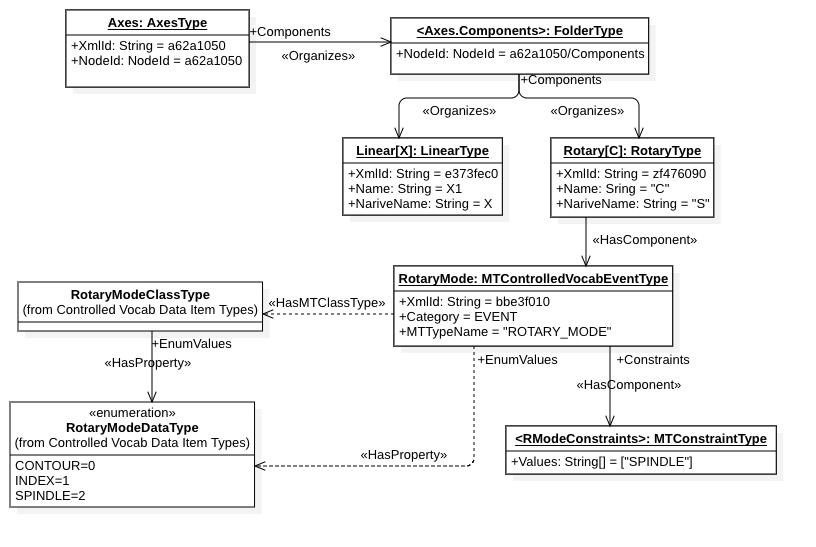
\includegraphics[width=1.0\textwidth]{diagrams/mtconnect-mapping/rotary-c-rotary-mode.png}
    \caption{Rotary[C] Axis RotaryMode DataItem}
    \label{fig:rotary-c-rotary-mode}
\end{figure}

\FloatBarrier

\begin{figure}[ht]
    \centering
    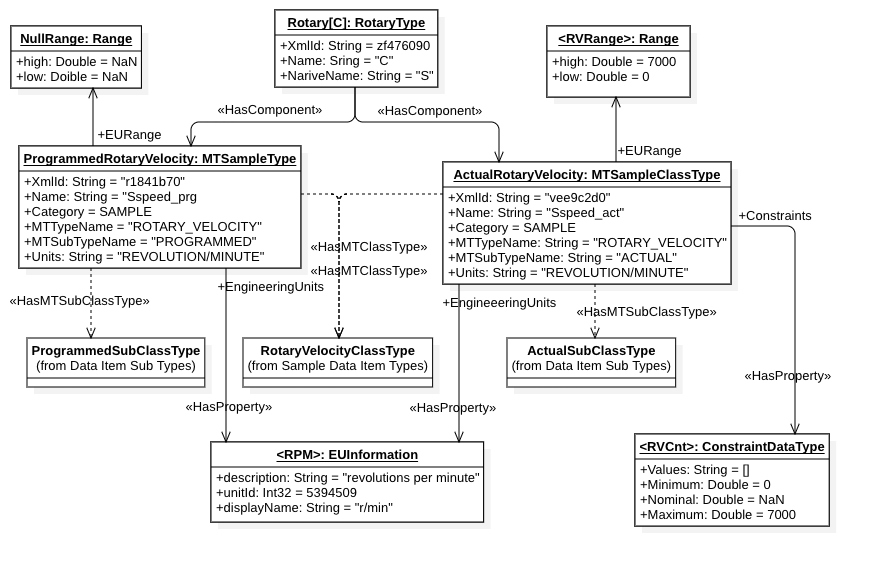
\includegraphics[width=1.0\textwidth]{diagrams/mtconnect-mapping/rotary-c-rotary-velocity.png}
    \caption{Rotary[C] Axis RotaryVelocity DataItem}
    \label{fig:rotary-c-rotary-velocity}
\end{figure}

Figure~\ref{fig:rotary-c-rotary-velocity} corresponds to Lines~\ref{line:programmed-rotary-velocity}-\ref{line:actual-rotary-velocity} of Figure~\ref{fig:rotary-c-rotary-velocity}--the two rotary velocity data items differentiated by their \xmlattribute{subType}s of \texttt{ACTUAL} and \texttt{PROGRAMMED}. In this case they share many of the same property values. The \mtterm{HasMTSubClassType} references the \mtuatype{ActualSubClassType} and the \mtuatype{ProgrammedSubClassType} respectively.

In the case of the \texttt{ActualRotaryVelocity} object, it has an additional constraint that specifies that the maximum spindle speed is 7000 RPM. This is given with the \mtuadatatype{ConstraintDataType}. These values are also reflected in the EURange associated with the two data items. \texttt{ProgrammedRotaryVelocity} references a \texttt{NullRange} where the \uaterm{high} and \uaterm{low} are both set to NaN, and the \texttt{ActualRotaryVelocity} references an \uaterm{EURange} where the \uaterm{high} and \uaterm{low} are the same as the \mtterm{Maximum} and \mtterm{Minimum} of the \mtuadatatype{ConstraintDataTyp} respectively. 

\FloatBarrier

Figure~\ref{fig:rotary-c-load} represents the \dataitem{Load} \mtterm{DataItem} for Listing~\ref{lst:rotary-c-example} Line~\ref{line:rotary-c-load} as an example of a \mtuatype{MTSampleType} where the \uaterm{EngineeringUnits} are not given in the \uaterm{UNECE} set and the \uaterm{unitId} is -1 and the \uaterm{namespaceUri} is set to the MTConnect specific units. The EURange is defined as the NullRange as was done for the \texttt{ProgrammedRotaryVelocity}.

\begin{figure}[ht]
    \centering
    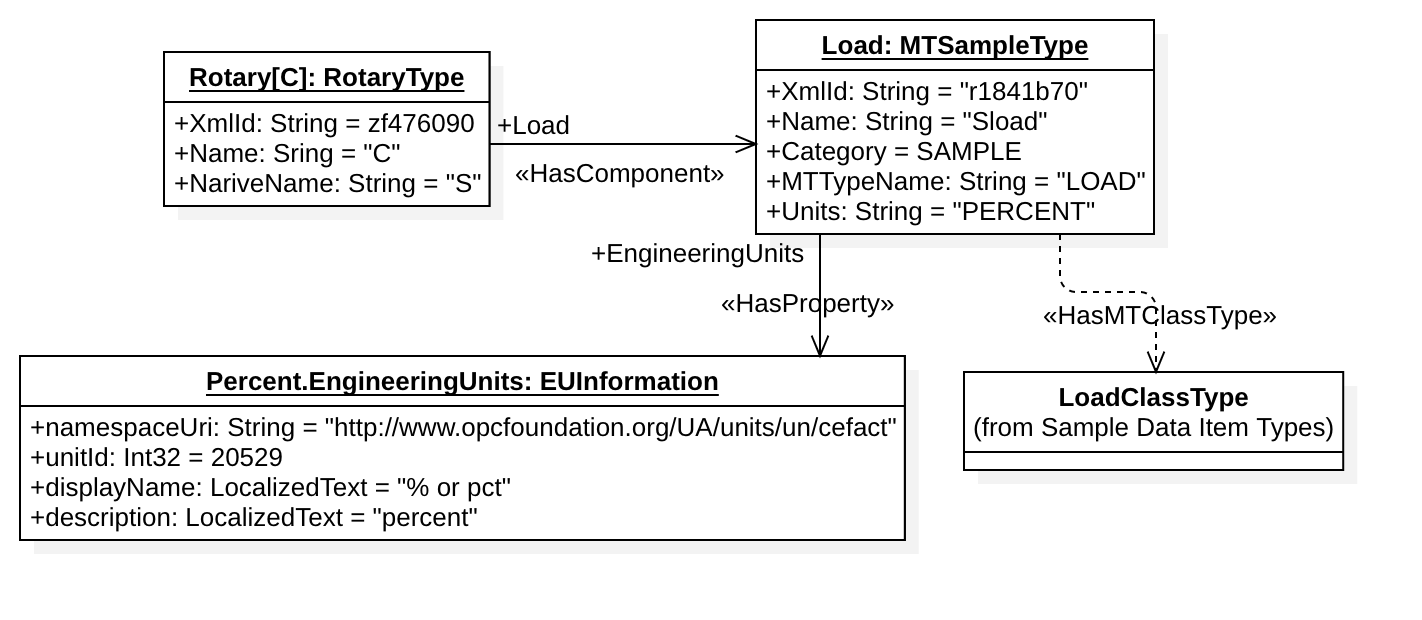
\includegraphics[width=1.0\textwidth]{diagrams/mtconnect-mapping/rotary-c-load.png}
    \caption{Rotary[C] Axis Load DataItem}
    \label{fig:rotary-c-load}
\end{figure}

\FloatBarrier

Figure~\ref{fig:rotary-c-amperage} illustrates the \mtterm{Amperage} \mtterm{DataItem} corresponding to the Listing~\ref{lst:rotary-c-example} Lines~\ref{line:rotary-c-amperage}-\ref{line:rotary-c-amperage-condition}. Unlike the previous example of a MTConnect \mtterm{Condition} relating to the MTConnect \mtterm{Component}, the \xmlelement{Source} element under the \xmlelement{DataItem} references the \mtterm{DataItem} with \xmlattribute{type} \dataitem{AMPERAGE}. When the \mtterm{source} refers to a \mtterm{DataItem} that is part of the same MTConnect \mtterm{Component}, the UA \uaterm{Variable} is given a \uaterm{Reference} \uaterm{HasEventSource} from the \mtterm{RotaryType} (Rotary[C]) and a \uaterm{HasCondition} \uaterm{Reference} is created beteen the \uaterm{Variable} to the \mtterm{MTConditionType}.

As stated above, the \uaterm{HasNotifier} \uaterm{References} must be established between all \mtterm{Components} back to the \mtuatype{MTDeviceType} that has a reference from the \uaterm{Server}. The \texttt{MotorAmperage} and \texttt{MotorAmperageCondition} demonstrate the naming rule where the Composition type is converted to \textit{PascalCase} and then prepended to the \mtterm{DataItem} \xmlattribute{type}. 

\begin{figure}[ht]
    \centering
    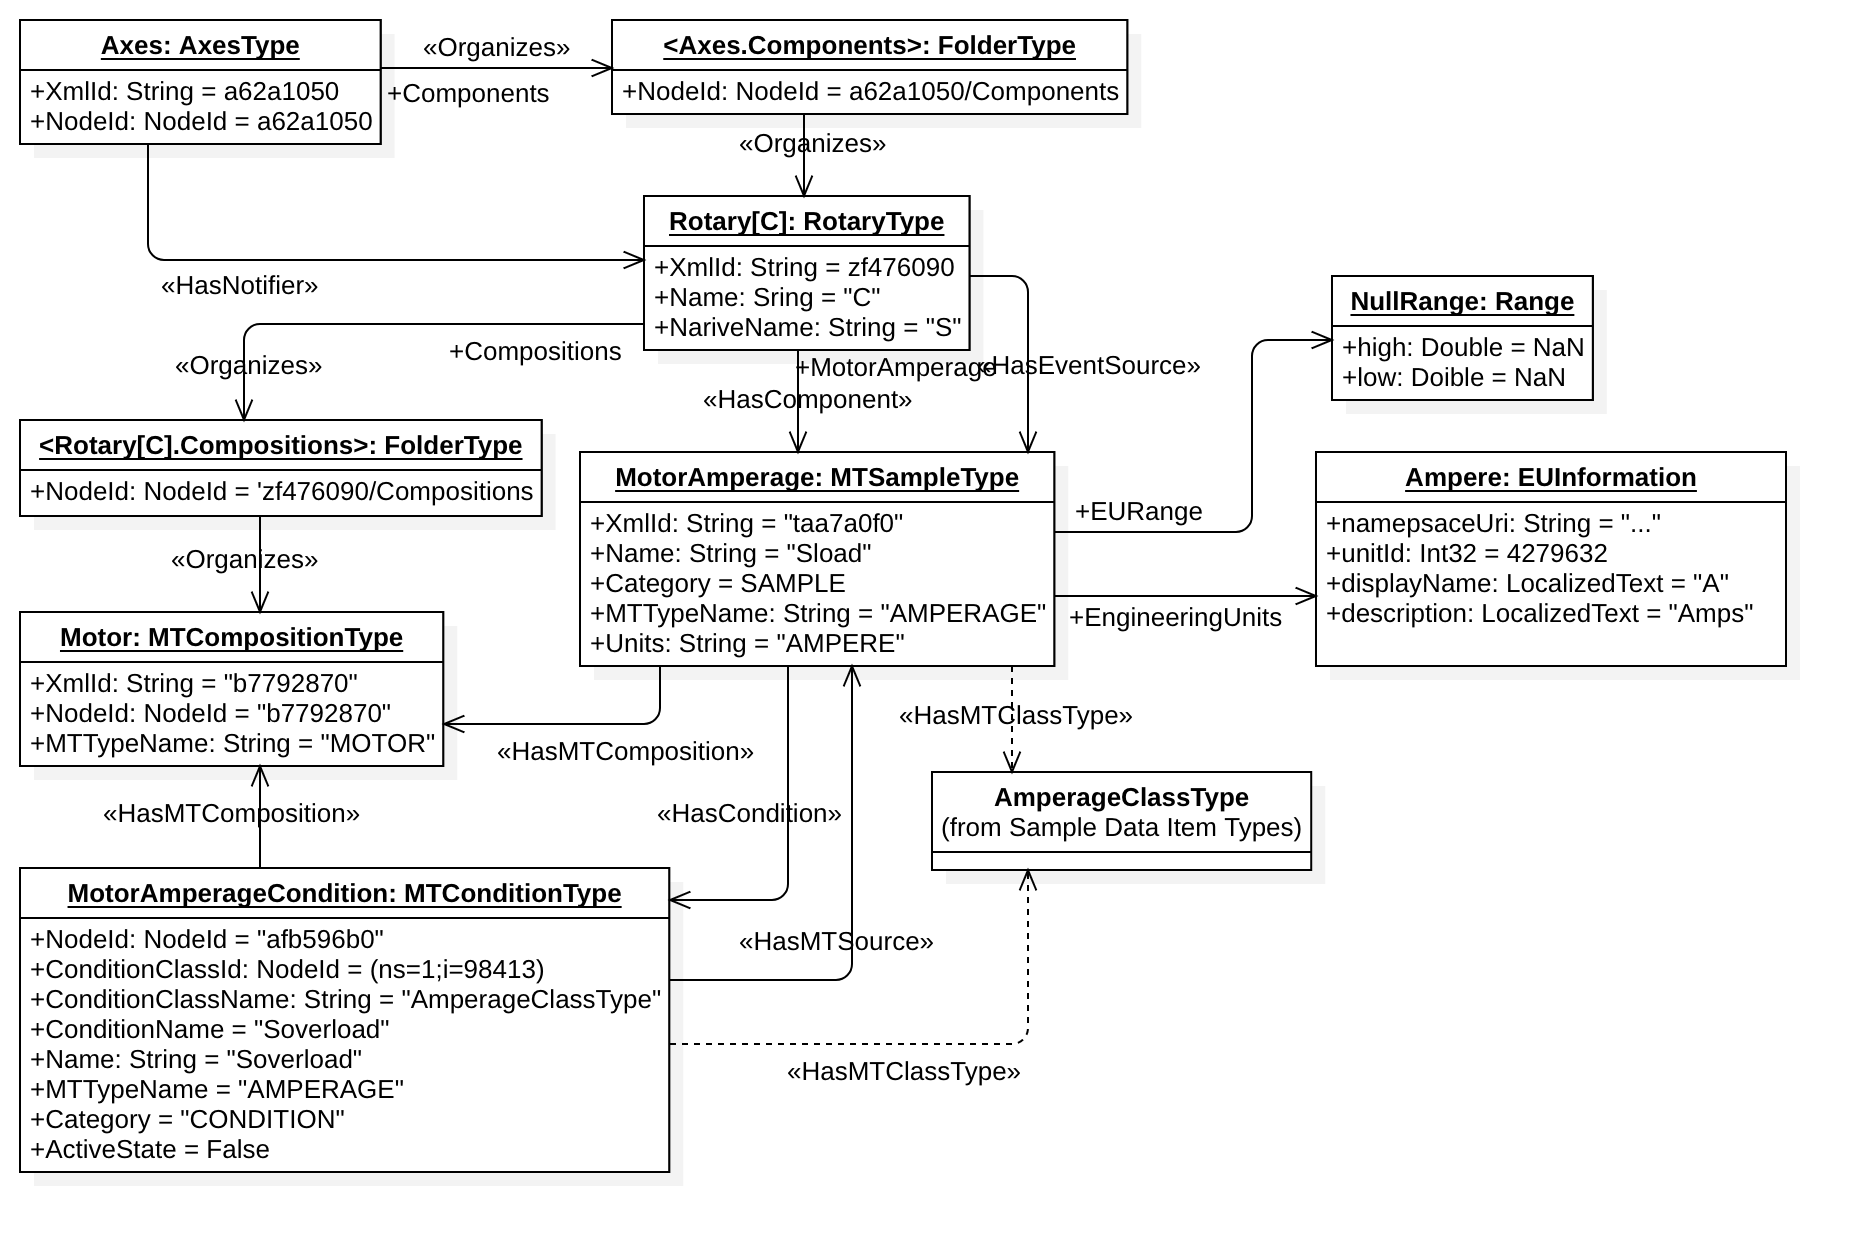
\includegraphics[width=1.0\textwidth]{diagrams/mtconnect-mapping/rotary-c-amperage.png}
    \caption{Rotary[C] Axis Motor Amperage DataItem}
    \label{fig:rotary-c-amperage}
\end{figure}

\FloatBarrier

\paragraph{\element{Controller} and \element{Path} \mtterm{Component}s}

In MTConnect, the \mtterm{Controller} component represents the control system of the machine. This includes both the PLC (Programmable Logic Controller) and the CNC (Computerized Numerical Controller) of the machine. In a CNC machine tool, the CNC and PLC are often thought of as a single component of the machine since they both control the operation of the machine.

The MTConnect information model does not differentiate between the two controllers, but represents them as a common controller category with data items that apply to both. Within a controller, there can be multiple \mtterm{Path}s, each representing a set of coordinated motion. The \mtterm{Path} is optional if the \mtterm{Controller} is representing a simple machine with a PLC and no motion, such as a boiler or oven. This is covered in MTConnect Part 2 \cite{MTCPart2}.

\begin{lstlisting}[firstnumber=last,%
    caption={Controller and Path Components and Their Data Items},label={lst:controller-component}]
        <Controller id="p5add360">
          <DataItems>
            <DataItem id="x7ca94e0" type="EMERGENCY_STOP" category="EVENT" name="estop"/>
            <DataItem id="m17f1750" type="MESSAGE" category="EVENT"/>
          </DataItems>
          <Components>
            <Path id="a4a7bdf0" name="P1">
              <DataItems>
                <DataItem id="if36ff60" type="CONTROLLER_MODE" category="EVENT"/>
                <DataItem id="a01c7f30" type="EXECUTION" category="EVENT"/>
                <DataItem id="k8dd9030" type="PROGRAM" category="EVENT"/>
                <DataItem id="r63f9b10" type="CONTROLLER_MODE_OVERRIDE" subType="OPTIONAL_STOP" category="EVENT"/>
                <DataItem id="a557d330" type="LOGIC_PROGRAM" category="CONDITION"/>
                <DataItem id="a5b23650" type="MOTION_PROGRAM" category="CONDITION"/>
                <DataItem id="bbafe670" type="LINE" category="EVENT"/>
                <DataItem id="d2e9e4a0" type="PART_COUNT" category="EVENT">
                  <InitialValue>1</InitialValue>
                </DataItem>
                <DataItem id="r186cd60" type="PATH_POSITION" category="SAMPLE" units="MILLIMETER_3D"/>
              </DataItems>
            </Path>
          </Components>
        </Controller>
\end{lstlisting}

The \mtterm{Controller} has two \mtterm{DataItems}, \mtterm{Message} and \mtterm{EmergencyStop} as shown in Figure~\ref{fig:controller-component}. The \mtuatype{MTMessageType} is of special note since it is not a \uaterm{VariableType}, but it is an \uaterm{EventType} and decended from the \uaterm{SystemEventType} class described in \cite{UAPart5}. {\color{red} Does the message require a special relation like the Condition and the HasCondition reference?}

\begin{figure}[ht]
    \centering
    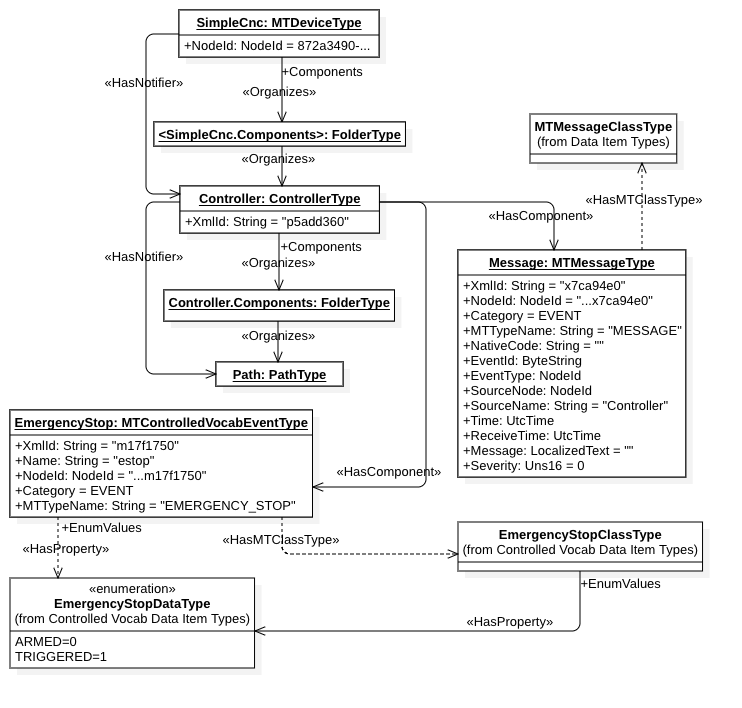
\includegraphics[width=1.0\textwidth]{diagrams/mtconnect-mapping/controller-component.png}
    \caption{Controller Component and Data Items}
    \label{fig:controller-component}
\end{figure}

Figure~\ref{fig:path-component} illustrates the \mtterm{Path} component. Many of the \mtterm{DataItems} types have been covered in prior examples, so the \mtterm{Path} will only focus on the \mtterm{DataItems} that have differentiated features. Those \mtterm{DataItem}s will be represented without additional properties or relations.

The \dataitem{PATH_POSITION} is mapped to the \mtuatype{MTThreeSpaceSampleType} that represents a spacial coordinate in three space ($\mathbb{R}^{3}$) with each coordinate being giving in millimeters. The EngineeringUnits for this type will therefor always be mapped to MMT in the UNECE conventions.

The \mtuatype{MTThreeSpaceSampleType} uses the \mtuatype{ThreeSpacePositionDataType} that contains an \mtterm{X, Y, and Z} \uaterm{Field}. If one of the dimensions cannot be provided, it must be set to \uaterm{NaN}.

The two \mtterm{Conditions} in this component capable of branching. The model will use the \uaterm{BranchId} in this case. This occurs when there are multiple simultaneous problems with either the logic or motion program in the controller. These cases will be discussed in the section on the streaming data.

\begin{figure}[ht]
    \centering
    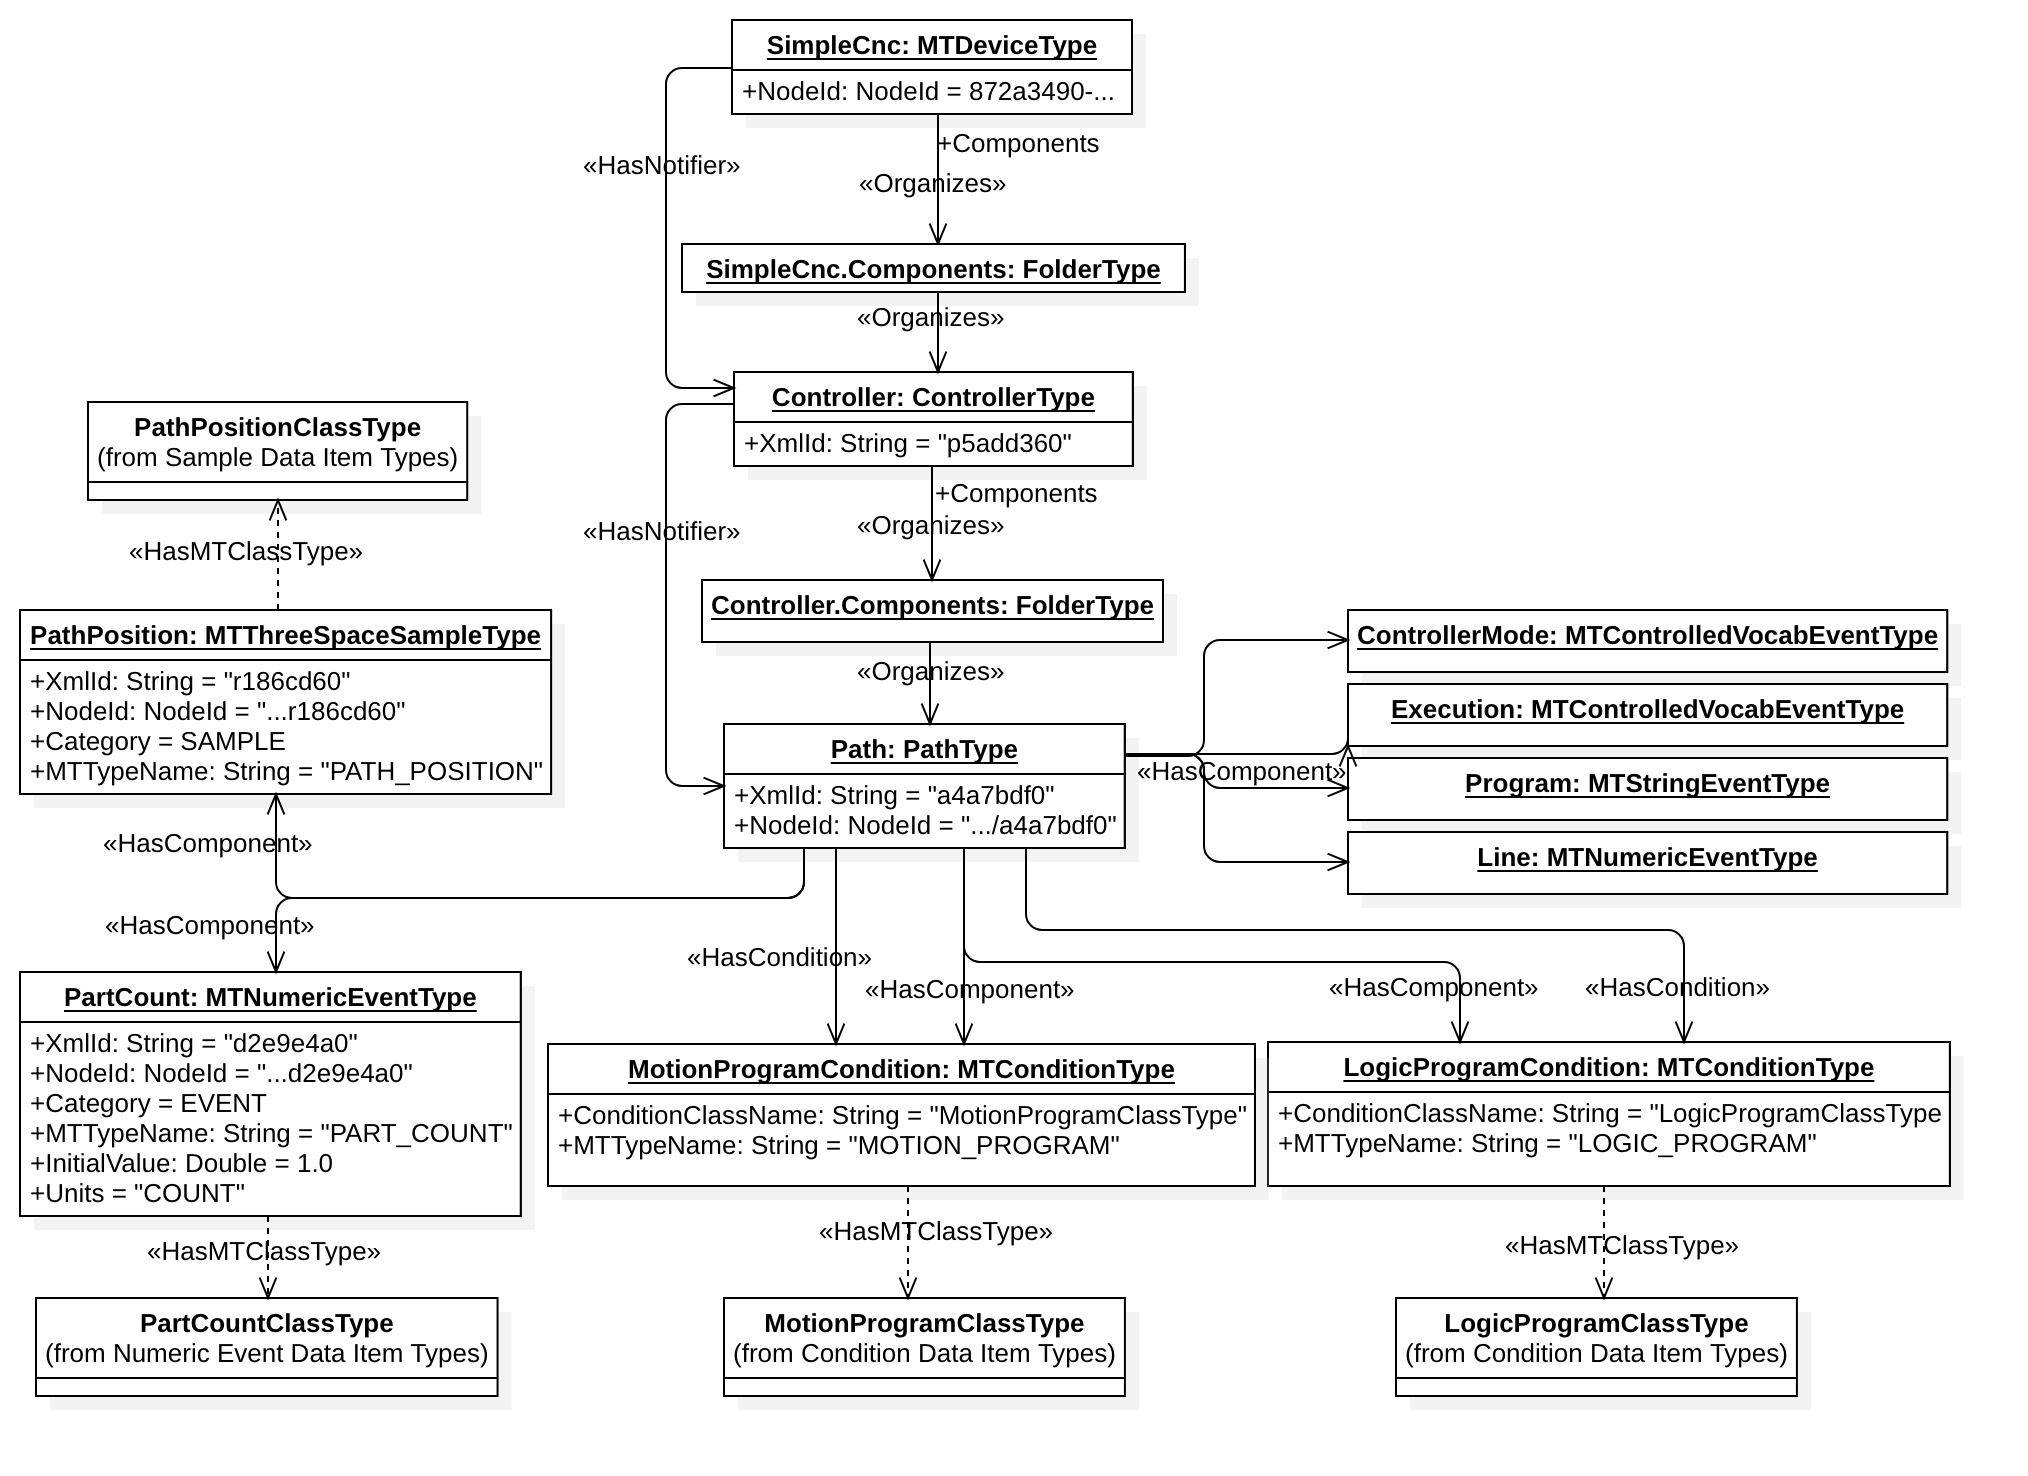
\includegraphics[width=1.0\textwidth]{diagrams/mtconnect-mapping/path-component.png}
    \caption{Path Component and Data Items}
    \label{fig:path-component}
\end{figure}

\FloatBarrier

\paragraph{\xmlelement{Electric} \mtterm{System} of the \xmlelement{Device}}

The following example is the \xmlelement{Electric} system of the machine. The top level \xmlelement{Systems} component is an organizational component, similar to an \uaterm{Folder} that collects \mtterm{Components} that are central to a function in the device. The \uaterm{Electric} component represents sensor data with some of the more advanced capabilities of the MTConnect standard. The \xmlelement{Electric} component demonstrate the use of a \xmlelement{Sensor} and \xmlelement{Configuration}.

\begin{lstlisting}[firstnumber=last,,escapechar=|,%
    caption={Electrical System and Sensor Configuration},label={lst:electric-system}]
        <Systems id="if618500">
          <Components>
            <Electric id="afb91ba0">
              <DataItems>
                <DataItem id="x52ca7e0" name="ptemp" type="TEMPERATURE" category="SAMPLE" units="CELSIUS">  |\label{line:electric-temp-60}|
                  <Filters>
                    <Filter type="PERIOD">60</Filter>
                  </Filters>
                </DataItem>
                <DataItem id="r1e58cf0" name="pvolt" type="VOLTAGE" category="SAMPLE" units="VOLT"> |\label{line:electric-voltage-10}|
                  <Filters>
                    <Filter type="MINIMUM_DELTA">10</Filter>
                  </Filters>
                </DataItem>
                <DataItem id="tc9edc70" name="pampts" type="VOLT_AMPERE" category="SAMPLE" units="VOLT_AMPERE" representation="TIME_SERIES" sampleRate="100"/>  |\label{line:electric-voltage-ampere}|
                <DataItem id="e25c1130" name="pamp" type="AMPERAGE" category="SAMPLE" units="AMPERE"/>  |\label{line:electric-amperage}|
                <DataItem id="qb9212c0" type="AMPERAGE" category="SAMPLE" units="AMPERE" statistic="AVERAGE">  |\label{line:electric-average-amperage}|
                  <ResetTrigger>ACTION_COMPLETE</ResetTrigger>
                </DataItem>
                <DataItem id="o63fcd30" name="ppfact" type="POWER_FACTOR" category="SAMPLE" units="PERCENT" />
                
                 <DataItem id="b4bb7110" type="AMPERAGE" category="CONDITION" name="poverload">
                   <Source dataItemId="e25c1130"/>
                 </DataItem>
                 <DataItem id="c82e32f0" type="TEMPERATURE" category="CONDITION" name="povertemp">
                   <Source dataItemId="x52ca7e0"/>
                 </DataItem>
              </DataItems>
\end{lstlisting}

In the first set of data items from Listing~\ref{lst:electric-system} as shown in Figure~\ref{fig:electric-system}, the first data item on line~\ref{line:electric-temp-60} has a period filter that is represented in the OPC UA \uaterm{Object} Temperature as a \mtterm{PeriodFilter} \uaterm{Property} with a value of 60.0. The period filters only recognize changes to data if the change after a period of the given value, in this case 60 seconds. This will only publish changed data every minute in this instance.

The following \mtterm{DataItem} on line~\ref{line:electric-voltage-10} has a \mtterm{Filter} using a \mtterm{MINIUM_DELTA} that is represened as a \mtterm{MinimumDeltaFilter} in the UA \uaterm{Object} reprenenting the \mtterm{MTSampleType} Voltage. The \mtterm{MinimumDelta} represents the smallest amount of change before the change is reported. In this case the minimum change is 10 volts. Changes smaller than 10 volts will not be reported for this data item.

\begin{figure}[ht]
    \centering
    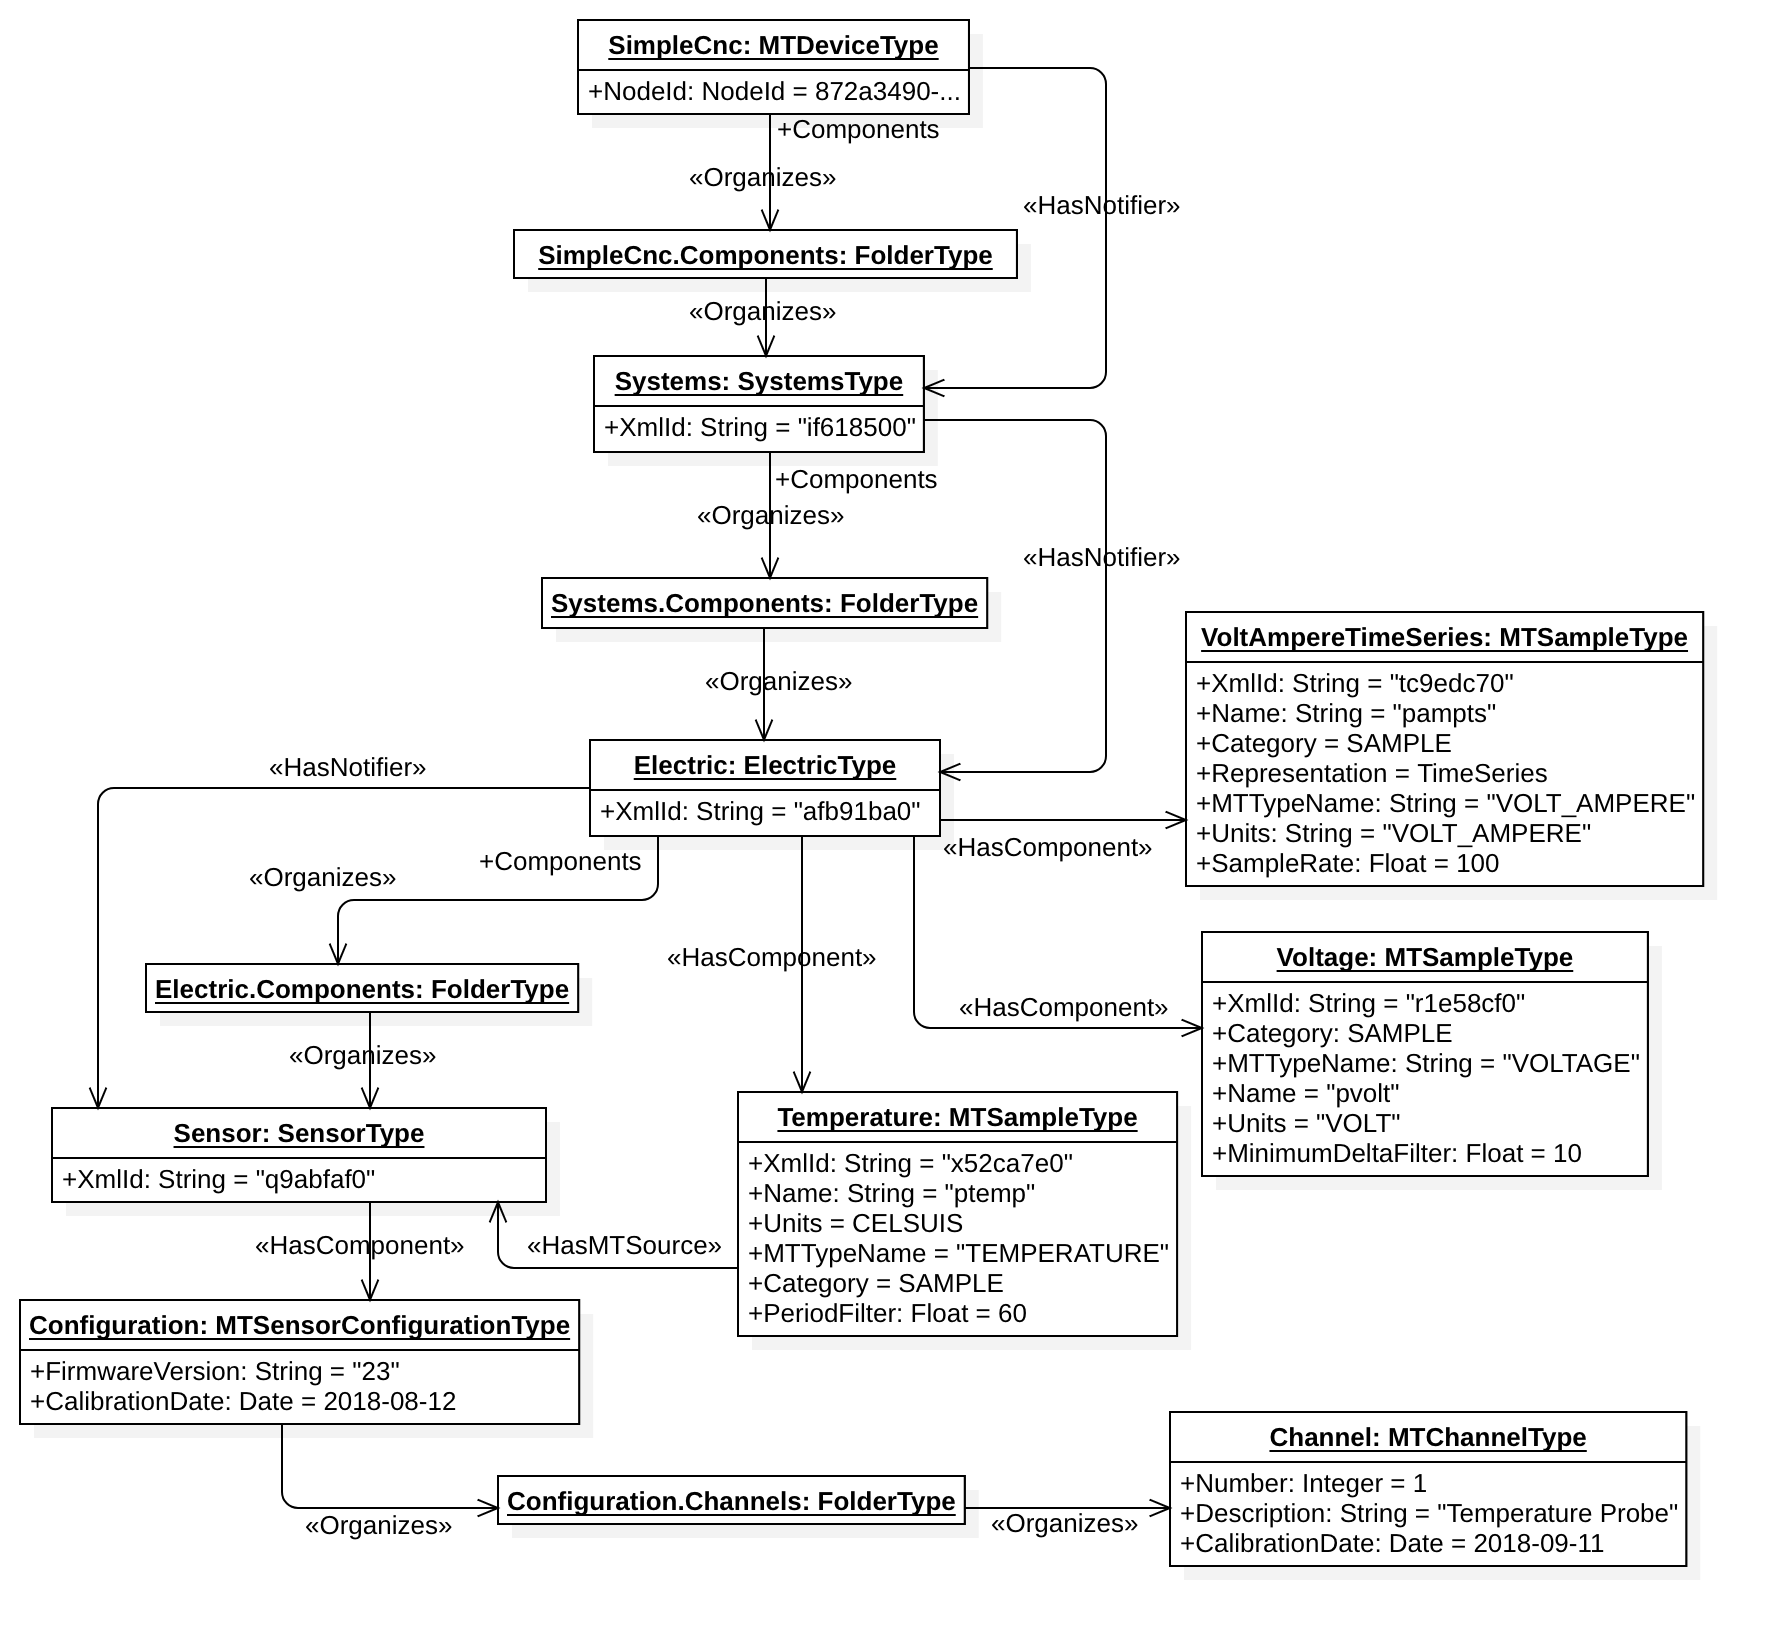
\includegraphics[width=1.0\textwidth]{diagrams/mtconnect-mapping/electric-system.png}
    \caption{Electric System Component}
    \label{fig:electric-system}
\end{figure}


\FloatBarrier

\begin{lstlisting}[firstnumber=last,%
    caption={Electrical System Sensor Configuration},label={lst:sensor-component}]
              <Components>
                <Sensor id="q9abfaf0">
                  <Configuration>
                    <SensorConfiguration>
                      <FirmwareVersion>23</FirmwareVersion>
                      <CalibrationDate>2018-08-12</CalibrationDate>
                      <Channels>
                        <Channel number="1">
                          <Description>Temperature Probe</Description>
                          <CalibrationDate>2018-09-11</CalibrationDate>
                        </Channel>
                      </Channels>
                    </SensorConfiguration>
                  </Configuration>
                </Sensor>              
              </Components>
            </Electric>
          </Components>
        </Systems>
\end{lstlisting}

\subsection{MTConnect Streaming Data}

MTConnect separates out the the streaming updates to the values of the data from the meta-data describing the semantic meaning of the data. This is covered in detail in \cite{MTCPart3}. The XML document also contains protocol information which will be ignored for handling of the streaming data. 

The \mtterm{HTTP REST} protocol provides both a snapshot and time series data from the \mtterm{MTConnect Agent} that is collected from the \mtterm{Device}s. Each entry is time-stamped and is given a sequence number that indicates the arrival order across all devices whose information is aggregated in the \mtterm{MTConnect Agent}.

The following section provides the rules and mechanism to take data from the MTConnect stream and represent as a series of updates to the \uaterm{Variables} and generate \uaterm{Events} for the \mtterm{MTConditionType} and \mtterm{MTMessageType}.

\begin{lstlisting}[firstnumber=1,escapechar=|,%
    caption={Streams Header},label={lst:streams-header}]
<?xml version="1.0" encoding="UTF-8"?>
<MTConnectStreams xmlns="urn:mtconnect.org:MTConnectStreams:1.4" xmlns:xsi="http://www.w3.org/2001/XMLSchema-instance" xsi:schemaLocation="urn:mtconnect.org:MTConnectStreams:1.4 ./schema/MTConnectStreams_1.4.xsd">
	<Header version="1.4.0" creationTime="2018-10-31T21:00:01Z" nextSequence="43124" lastSequence="44221" firstSequence="1" instanceId="1541045065" sender="localhost" bufferSize="131072"/>
	<Streams>
    <DeviceStream name="SimpleCnc" uuid="872a3490-bd2d-0136-3eb0-0c85909298d9">    
\end{lstlisting}

Listing~\ref{lst:streams-header} root element \xmlelement{MTConnectStreams} contains the standard namespace declarations for MTConnect and XMLSchema. If additional namespaces are noted, they should be added as additional namespaces in the OPC UA \uaterm{Namespace} as well. The streams document begins with a Header with protocol information that represents the version of the standard being references and the store-and-forward buffer sequence numbers. \cite{MTCPart1} provides information on the interaction with the \mtterm{Agent} and the proper sequence of requests to receive a conriguous stream of data.

\begin{lstlisting}[firstnumber=last,escapechar=|,%
    caption={Comoonent Stream},label={lst:component-stream}]
      <ComponentStream componentId="e373fec0" component="Linear" name="X1" nativeName="X"> |\label{line:component-stream}|
        <Samples>
          <Position sequence="131" timestamp="2018-10-31T20:33:11Z" dataItemId="dcbc0570" name="Xpos">UNAVAILABLE</Position> |\label{line:pos-unavilable}|
          <Position sequence="794" timestamp="2018-10-31T20:47:09Z" dataItemId="dcbc0570" name="Xpos">205.23</Position> |\label{line:pos-795}|
        </Samples>
      </ComponentStream>
\end{lstlisting}

MTConnect only reports data when it changes. Each change is assigned a monotonically increasing sequence number when it arrives at the \textit{MTConnect Agent}. MTConnect organizes flattens the structure when reporting data and organizes it by \mtterm{Component} and \mtterm{Category}, this is shown in  Listing~\ref{lst:linear-component-stream} Line~\ref{line:component-stream}. When the data stream is initialized or when it disconnects, the MTConnect \mtterm{DataItem Value} is set to \texttt{UNAVAILABLE} as shown on Line~\ref{line:pos-unavilable}.

The sequence number indicates the arrival order in the \mtterm{Agent} and the \xmlattribute{timestamp} indicates the time the observation was made. The \xmlattribute{timestamp} will be used when setting the \uaterm{Variable} with the data that has arrived from the \mtterm{Device}. The data is only reported when it changes with the exception of \mtterm{DataItems} with the \mtterm{representation} of \texttt{DISCRETE} indicating that each value has a discrete meaning, such as a \mtterm{PartCount} where each count indicates an accrual of that many parts. {\color{red} It is unclear how to achieve this in OPC UA, possible with events as is being done with \mtuatype{MTMessageType}}.

The value of \texttt{UNAVAILABLE} will be translated to the OPC UA \uaterm{DataVariable} \uaterm{StatusCode} of \texttt{Bad_NotConnected} to indicate that the value of the data is currently unknown from the data source. 

The followiing examples provide the steps to translate from the \mtterm{MTConnectStreams} document to the OPC UA information model presented above.

\subsubsection{Samples}

The \mtterm{DataItems} with \mtterm{category} \dataitem{SAMPLE} are mapped to the \mtuatype{MTSampleType} which is a subtype of the \uaterm{AnalogItemType} \uaterm{DataVariable}. The numeric value of the sample sets the \uaterm{Variable} 

\begin{lstlisting}[firstnumber=last,escapechar=|,%
    caption={Linear Component Stream},label={lst:linear-component-stream}]
      <ComponentStream componentId="e373fec0" component="Linear" name="X1" nativeName="X"> |\label{line:component-stream}|
        <Samples>
          <Position sequence="794" timestamp="2018-10-31T20:47:09.1011Z" dataItemId="dcbc0570" name="Xpos">205.23</Position> |\label{line:pos-795}|
          <Position sequence="809" timestamp="2018-10-31T20:47:09.6021Z" dataItemId="dcbc0570" name="Xpos">206.23</Position> |\label{line:pos-809}|
        </Samples>
      </ComponentStream>
\end{lstlisting}

The OPC UA \uaterm{DataVariableType}s are monitored items and have three attribtues that are updated when the value changes. They are the \uaterm{Value} in the instance of the \uaterm{DataVariable}, the \uaterm{Time}, and the \uaterm{Quality}. When the value is given, not \texttt{UNAVAILABLE}, the \uaterm{Quality} will be set to the Status Code of \uaterm{Good}, the \uaterm{Time} will be set to the \xmlattribute{timestamp} attribute and the \uaterm{Value} set to the contents of the \xmlelement{CDATA} converted to a \mtterm{Double} precision value.

\subsubsection{String and Numeric Events}\label{sec:sting-numeric-events}

The \mtuatype{MTStringEventType} and \mtuatype{MTNumericEventType} \mtterm{DataItems} are managed in the same manner as the \mtuatype{MTSampleType} where the \uaterm{Value}, \uaterm{Quality}, and \uaterm{SourceTimestamp} are taken from the \xmlelement{CDATA}, \texttt{UNAVALAILABLE} state, and \xmlattribute{timestamp} respectively.

\begin{lstlisting}[firstnumber=last,escapechar=|,%
    caption={Path Component Stream},label={lst:path-component-stream}]
      <ComponentStream componentId="a4a7bdf0" component="Path" name="P1">
        <Events>
          <Program sequence="430" timestamp="2018-10-31T20:47:09Z" dataItemId="k8dd9030">O98877</Program> |\label{line:prog-430}|
          <PartCount sequence="630" timestamp="2018-10-31T20:57:09Z" dataItemId="d2e9e4a0">662</PartCount> |\label{line:pc-603}|
          <ControllerMode sequence="255" timestamp="2018-10-31T20:27:09Z" dataItemId="if36ff60">AUTOMATIC</ControllerMode> |\label{line:cmode-255}|

        </Events>
      </ComponentStream>
\end{lstlisting}

In Listing~\ref{lst:path-component-stream} on Line~\ref{line:prog-430}, the string value will be assiogned to the Program data item in the Path component. The following Line~\ref{line:pc-603} representing the part count will be converted to a numeric value, in this case an \uaterm{Int32} and assigned to the value.

All extended event types will be treated as \mtuatype{MTStringEventType}s since it can support any value. It will be the responsibility of the application to interpret the value.
 
\subsubsection{Controlled Vocabulary Events}

Controlled Vocabularies are represented as \mtuatype{MTControlledVocabEventType} which is a subtype of the \uaterm{MultiStateValueDiscreteType}. The \uaterm{MultiStateValueDiscreteType} requires an integer index to be used for the value, so the text given in MTConnect must be translated.

Referring to Listing~\ref{lst:path-component-stream} Line~\ref{line:cmode-255}, the values of the \texttt{CDATA} represent the allowed enumerations in the \mtuaenum{ControllerModeDataType} as shown in 
Table~\ref{table:example-ControllerModeDataType}. In this case the value from mtconnect is \texttt{AUTOMATIC} and is looked up in the associated \uaterm{EnumerationDataType} and the integer value is assigned to the \uaterm{Value} of the \mtuatype{MTControlledVocabEventType} instance, in this example the value will be \texttt{0} for \texttt{AUTOMATIC}.

\begin{table}[ht]
\centering 
  \caption{\texttt{ControllerModeDataType} Enumeration}
  \label{table:example-ControllerModeDataType}
\tabulinesep=3pt
\begin{tabu} to 6in {|l|r|} \everyrow{\hline}
\hline
\rowfont\bfseries {Name} & {Index} \\
\tabucline[1.5pt]{}
\texttt{AUTOMATIC} & \texttt{0} \\
\texttt{EDIT} & \texttt{1} \\
\texttt{MANUAL} & \texttt{2} \\
\texttt{MANUAL_DATA_INPUT} & \texttt{3} \\
\texttt{SEMI_AUTOMATIC} & \texttt{4} \\
\end{tabu}
\end{table} 

Tjhe \uaterm{SourceTimestamp} and \uaterm{Quality} will be handled as described in Section~\ref{sec:sting-numeric-events} for \mtterm{String and Numeric Events}.

\FloatBarrier

\subsubsection{Conditions}

Conditions are represnted by the \mtuatype{MTConditionType} that is a subtype of the \uaterm{ConditonType}. The MTConnect \mtterm{Conditions} are a representation of the transitional state of various alarms and reporting on the functioning of a \mtterm{Component} of the machine. There are three states for a conditon in MTConnect, they are \mtterm{Normal}, \mtterm{Warning}, and \mtterm{Fault} that have the semantic meaning \textit{operating normally}, \textit{a situation has been observed, but may self-correct}, and \textit{a failure has occured and needs manual intervention}. More information can be found in MTConnect \cite{MTCPart2} and \cite{MTCPart3} of the MTConnect Standard on Condition behavior.

The \mtuatype{MTConditionType} has a \uaterm{Property} called \texttt{ActiveState} that represents if there are any warnings or faults currently active. The \texttt{ActiveState} is an OPC UA \uaterm{TwoStateVariableType} defined in \cite{UAPart8}. When a Condition is \mtterm{Normal}, the \texttt{ActiveState} will be \texttt{False}, otherwise when either a \mtterm{Warning} or \mtterm{Fault} is present, the \texttt{ActiveState} will be \texttt{True}.

\begin{lstlisting}[firstnumber=last,escapechar=|,%
    caption={Rotary C Component Stream},label={lst:rotary-component-stream}]
      <ComponentStream componentId="zf476090" component="Rotary" name="C" nativeName="S">
        <Condition>
          <Normal sequence="201" timestamp="2018-10-31T20:34:19.9981Z" dataItemId="afb596b0" type="AMPERAGE" compositionId="b7792870" name="Soverload"/> |\label{line:amp-201}|
          <Warning sequence="503" timestamp="2018-10-31T20:45:19.9981Z" dataItemId="afb596b0" type="AMPERAGE" compositionId="b7792870" name="Soverload" qualifier="HIGH" nativeCode="MOT-WARN">Spindle Motor Warning</Warning> |\label{line:amp-503}|
          <Fault sequence="652" timestamp="2018-10-31T20:49:19.9981Z" dataItemId="afb596b0" type="AMPERAGE" compositionId="b7792870" name="Soverload" qualifier="HIGH" nativeCode="MOT-OVR">Spindle Motor Overload</Fault> |\label{line:amp-652}|
        </Condition>
\end{lstlisting}

The instance of the \mtuatype{MTConditionType} will contain the last state of the \mtterm{Condition} as most recently observed. Each time an MTConnect \mtterm{Condition} activates or deactivates, an \uaterm{Condition} \uaterm{Event} will be created associated with the instance if the \mtuatype{MTConditionType} \uaterm{NodeId}. 

The \uaterm{ConditionType} and \uaterm{EventType} properties will be set as follows:

\begin{itemize}
    \item \uaterm{EnableState} will be set as follows:
    \begin{itemize}
        \item If the \xmlelement{QName} is \xmlelement{Unavailable}, \uaterm{EnableState} is \uaterm{False}
        \item Otherwise, \uaterm{EnableState} is \uaterm{True}
    \end{itemize}
    \item \uaterm{Severity}:
    \begin{itemize}
        \item When \mtterm{Normal}, \uaterm{Severity} is 0.
        \item When \mtterm{Warning}, \uaterm{Severity} is 500.
        \item When \mtterm{Fault}, \uaterm{Severity} is 1000.
    \end{itemize}
    \item \uaterm{Retain}
    \begin{itemize}
        \item When \mtterm{Normal}, \uaterm{False}
        \item When \mtterm{Warning} or \mtterm{Fault}, \uaterm{True}
    \end{itemize}
    \item \uaterm{Message} set from the \xmlelement{CDATA}
    \item \uaterm{Time}, \xmlattribute{timestamp}
\end{itemize}

The remaining \uaterm{Properties} will be set from the XML attributes of the same name.

\begin{quote}
    \color{red} TODO: Need to handle branching based on \xmlattribute{nativeCode}.
\end{quote}

\subsubsection{Messages}

\begin{quote}
    \color{red} TODO: Messages are similar to conditions; they are events and they will have a similar duality. The message does not have state, but needs to have a meta data instance to reference. The instance can be mounted in the address space to serve as the NodeId for the Event.
\end{quote}


\subsection{Time Series Samples}
